\documentclass[12pt]{scrartcl}
\usepackage[version=4]{mhchem}
\usepackage{achemso}
\usepackage{graphicx}
\usepackage{float}
\usepackage[english]{babel}
\usepackage[T1]{fontenc}
\usepackage{setspace}
\usepackage{subcaption}
\usepackage{amsmath}

\renewcommand{\thepage}{S-\arabic{page}}
\begin{document}

\title{
\linespread{2.5} \fontsize {18}{8} \selectfont From the chemical bond to chemical reactivity: effects of electron (de)localization and Pauli exclusion in the \ce{H2} + \ce{H^.} atom transfer reaction\\[0.2in]
\fontsize {14}{8} \selectfont Supporting information\\[0.25in]
\fontsize {12}{8} \selectfont Shehan H. Fernando$^a$ and Alistair J. Sterling$^{a*}$\\[0.25in]
\fontsize{10}{8} \selectfont $^\text{a}$ Department of Chemistry and Biochemistry, University of Texas at Dallas, 800 W. Campbell road,  Richardson, Texas 75080-3021, United States\\[0.25in]
\fontsize{10}{8} \selectfont Email: Alistair.sterling@utdallas.edu
\date{}
}

\maketitle
\setstretch{1.15}



\section{2D Born--Oppenheimer potential energy surfaces and saddle point location}

The minimum energy path (MEP) traced on the Born--Oppenheimer potential energy surface (PES) the collinear \ce{H3}+\ce{H^.} (\ce{^2H3} doublet) atom transfer makes the backbone of our work. The CASSCF/aug-cc-pVTZ potential energy surface of this reaction was calculated by considering the whole valence space as active (CAS(3,3)). The tracing was done by the RBF interpolator function of SciPy\cite{scipy2020} and this trace is a smooth descent path compared to a path calculated using intrinsic reaction coordinate (IRC) method. The smoothness of the MEP is of high importance to electronic kinetic energy analysis (kinetic energy hereafter) as the kinetic energy is more sensitive to the fluctuations in the path than the total energy.\cite{slater1933,lowdin1959} We compared the saddle point of CASSCF surface with literature and it was noted the barrier height is overestimated.\cite{peterson2002} However, we are not aiming to calculate quantitatively accurate energy surfaces. It is sufficient if the qualitative nature of the surfaces are preserved. The qualitative correctness of the energy surfaces were verified by using the CCSDT method and the FIC-NEVPT2 implementation in ORCA 6.0.1\cite{neese2025}. The calculations were performed using Q-Chem 6.2.1\cite{qchem6} with the exception of NEVPT2 calculations performed using ORCA 6.0.1. The aug-cc-pVTZ\cite{dunning1992} basis set is used for all the calculations. 

\begin{figure}[H]
\centering
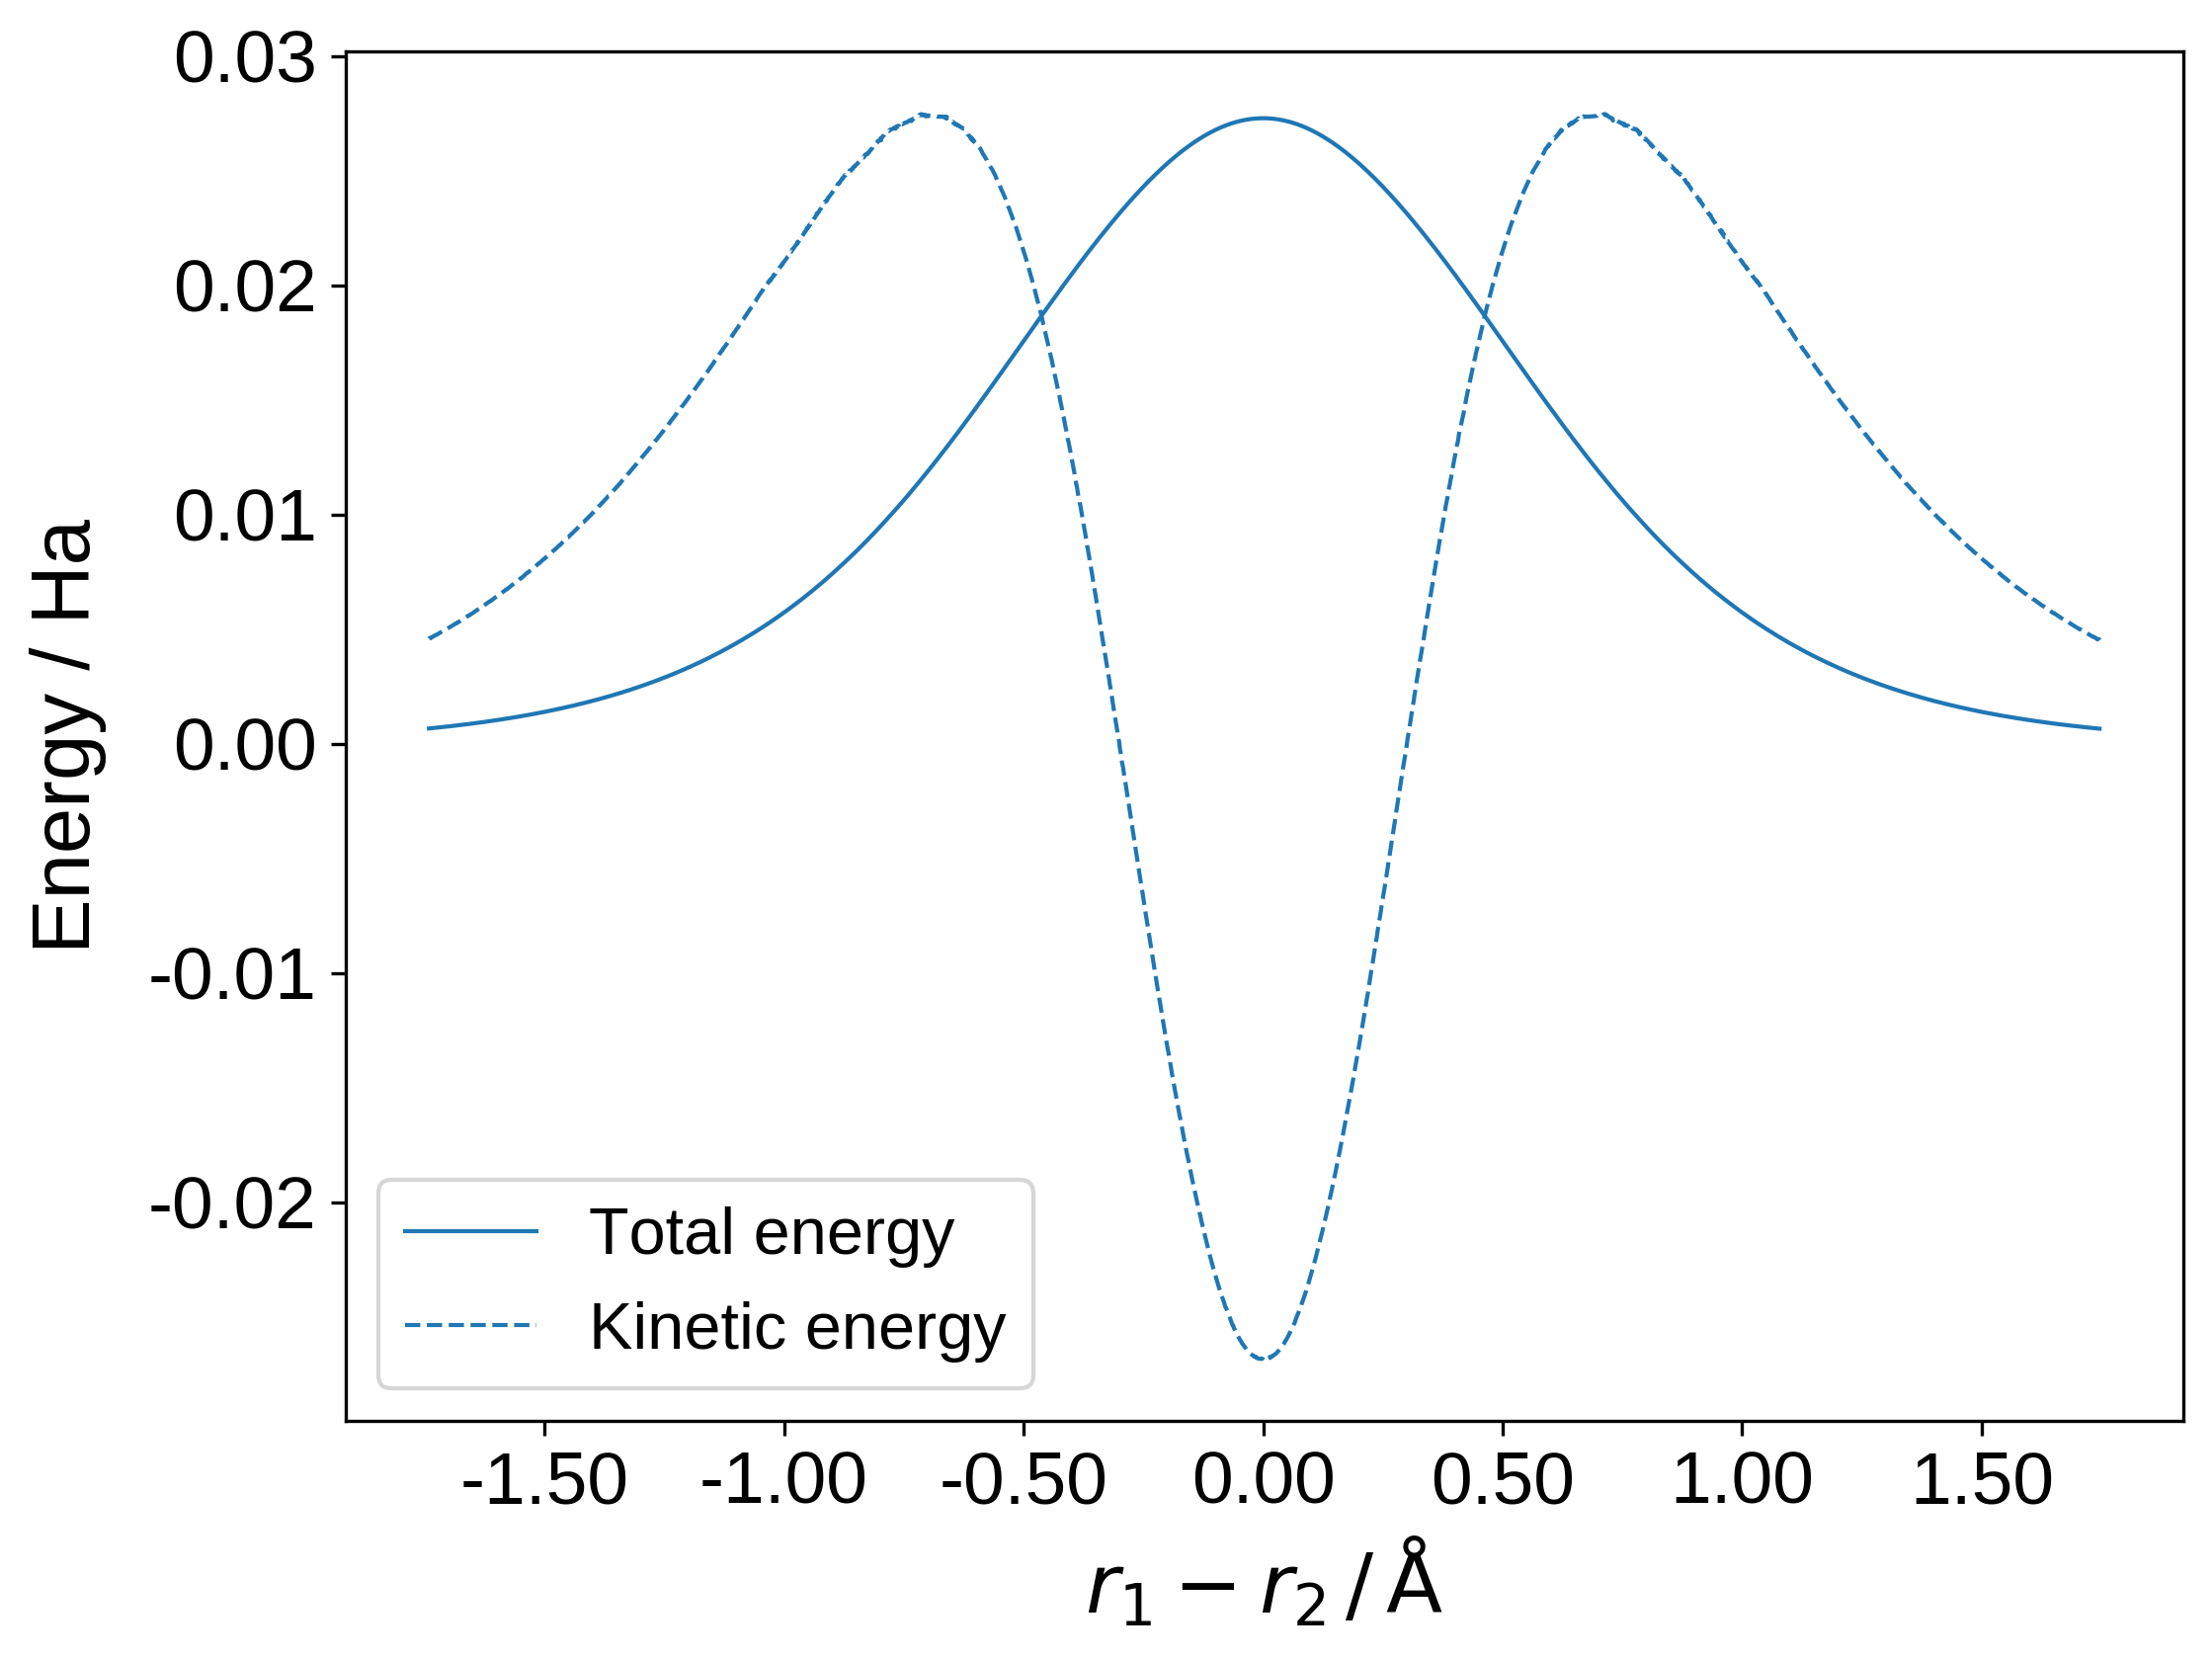
\includegraphics[width=0.62\textwidth]{images/doublet_ECA.png}
\caption{The kinetic energy composition of the collinear \ce{H3}+\ce{H^.} (\ce{^2H3} doublet) along the minimum energy path}
\end{figure}

\begin{figure}[H]
\centering
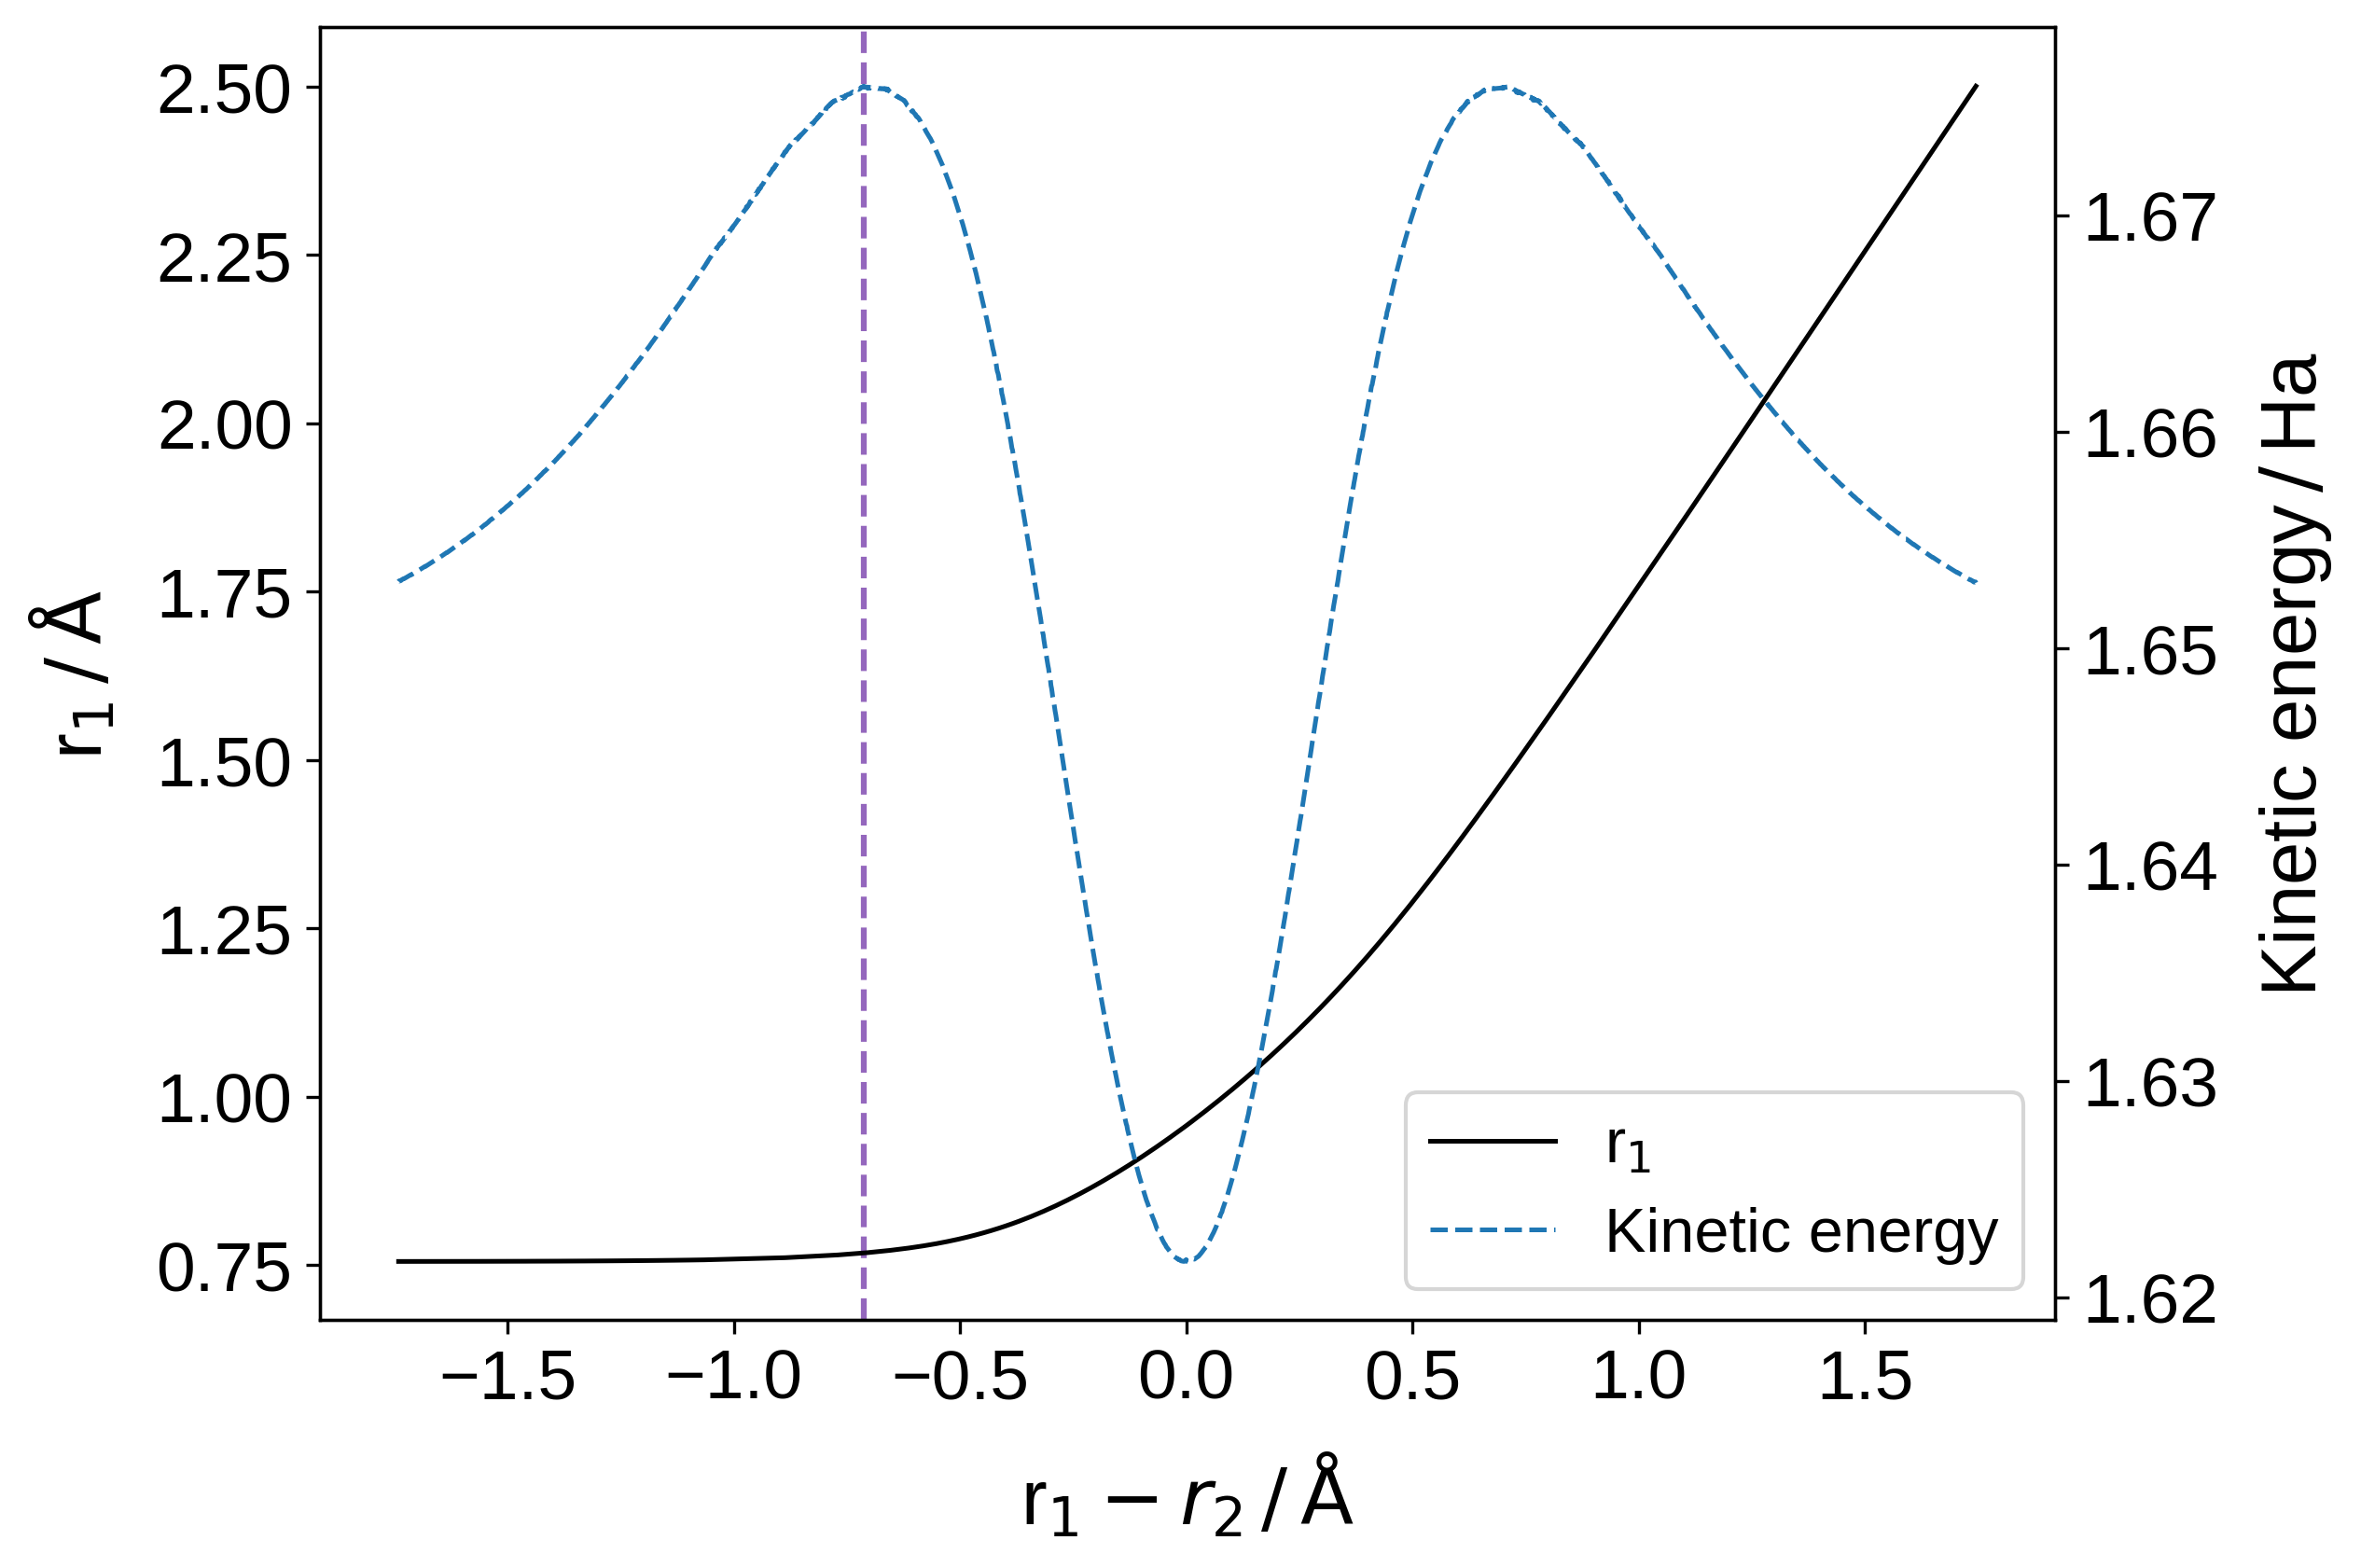
\includegraphics[width=0.7\textwidth]{images/BL_vsKE.png}
\caption{Geometric distortion of the \ce{H2} bond length overlaid with the kinetic energy of the \ce{^2H3}}
\end{figure}


\begin{figure}[H]
\centering
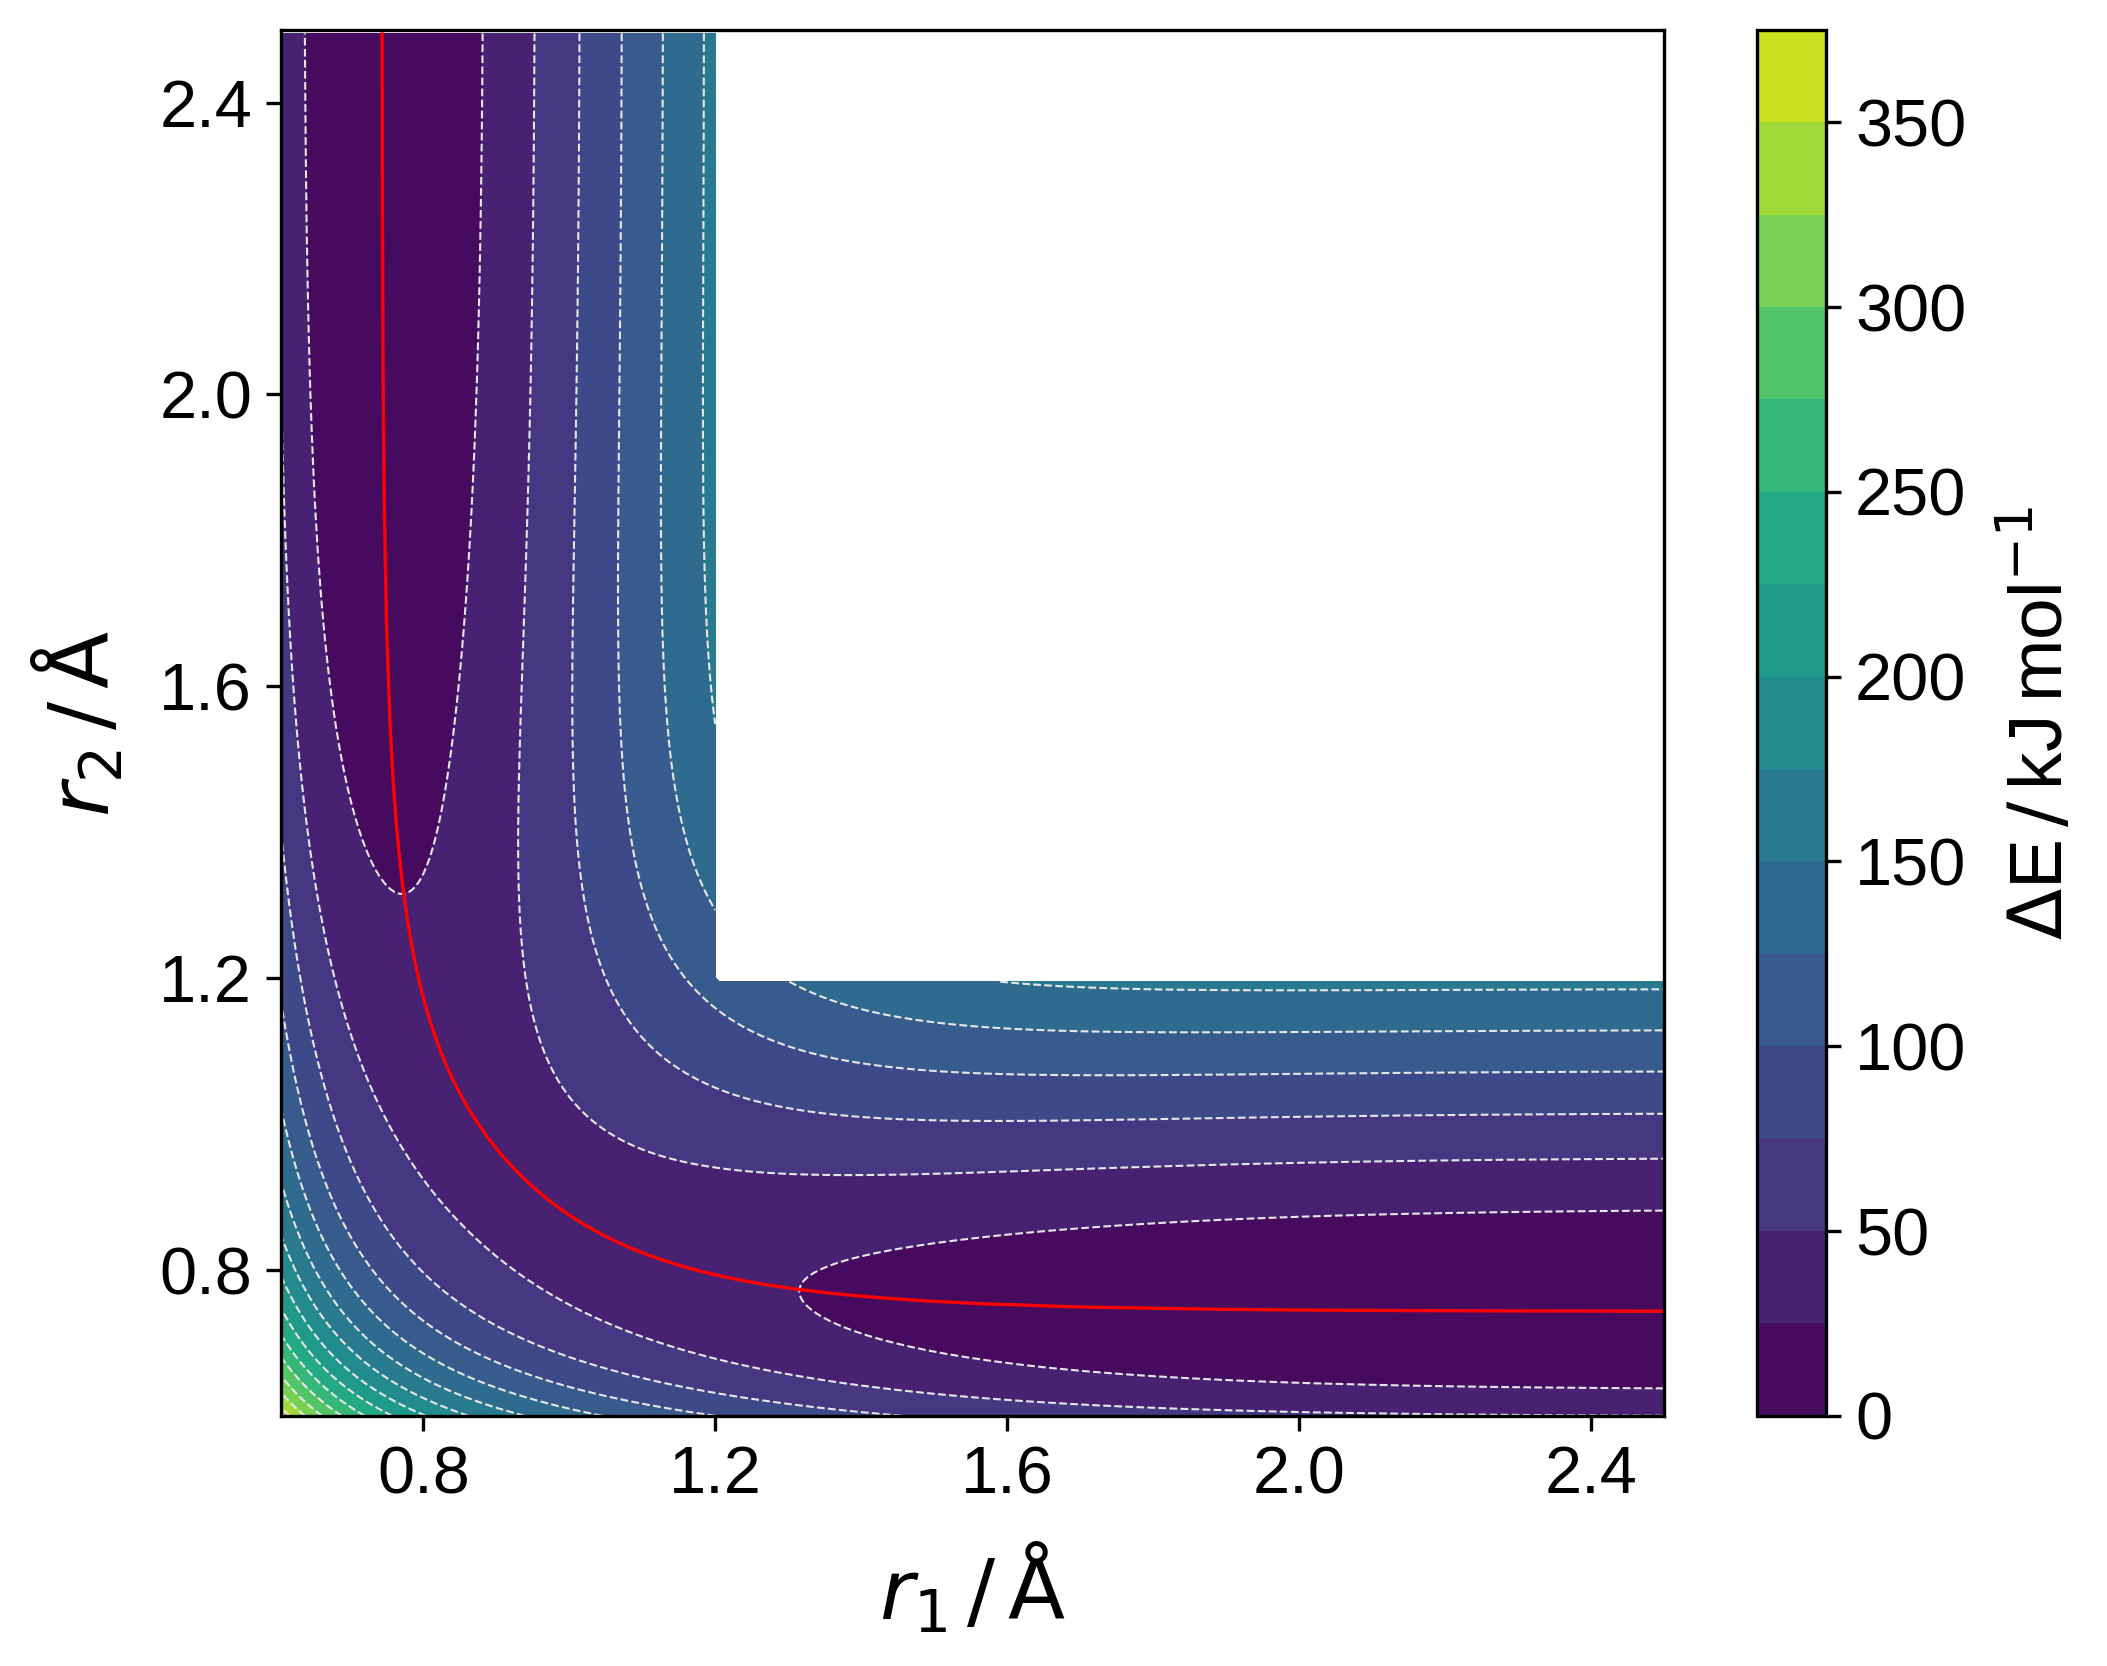
\includegraphics[width=0.62\textwidth]{images/PES_heat_map_ccsdt.png}
\caption{The 2D potential energy surface of the collinear \ce{^2H3} at CCSDT/aug-cc-pVTZ}
\end{figure}

\begin{figure}[H]
\centering
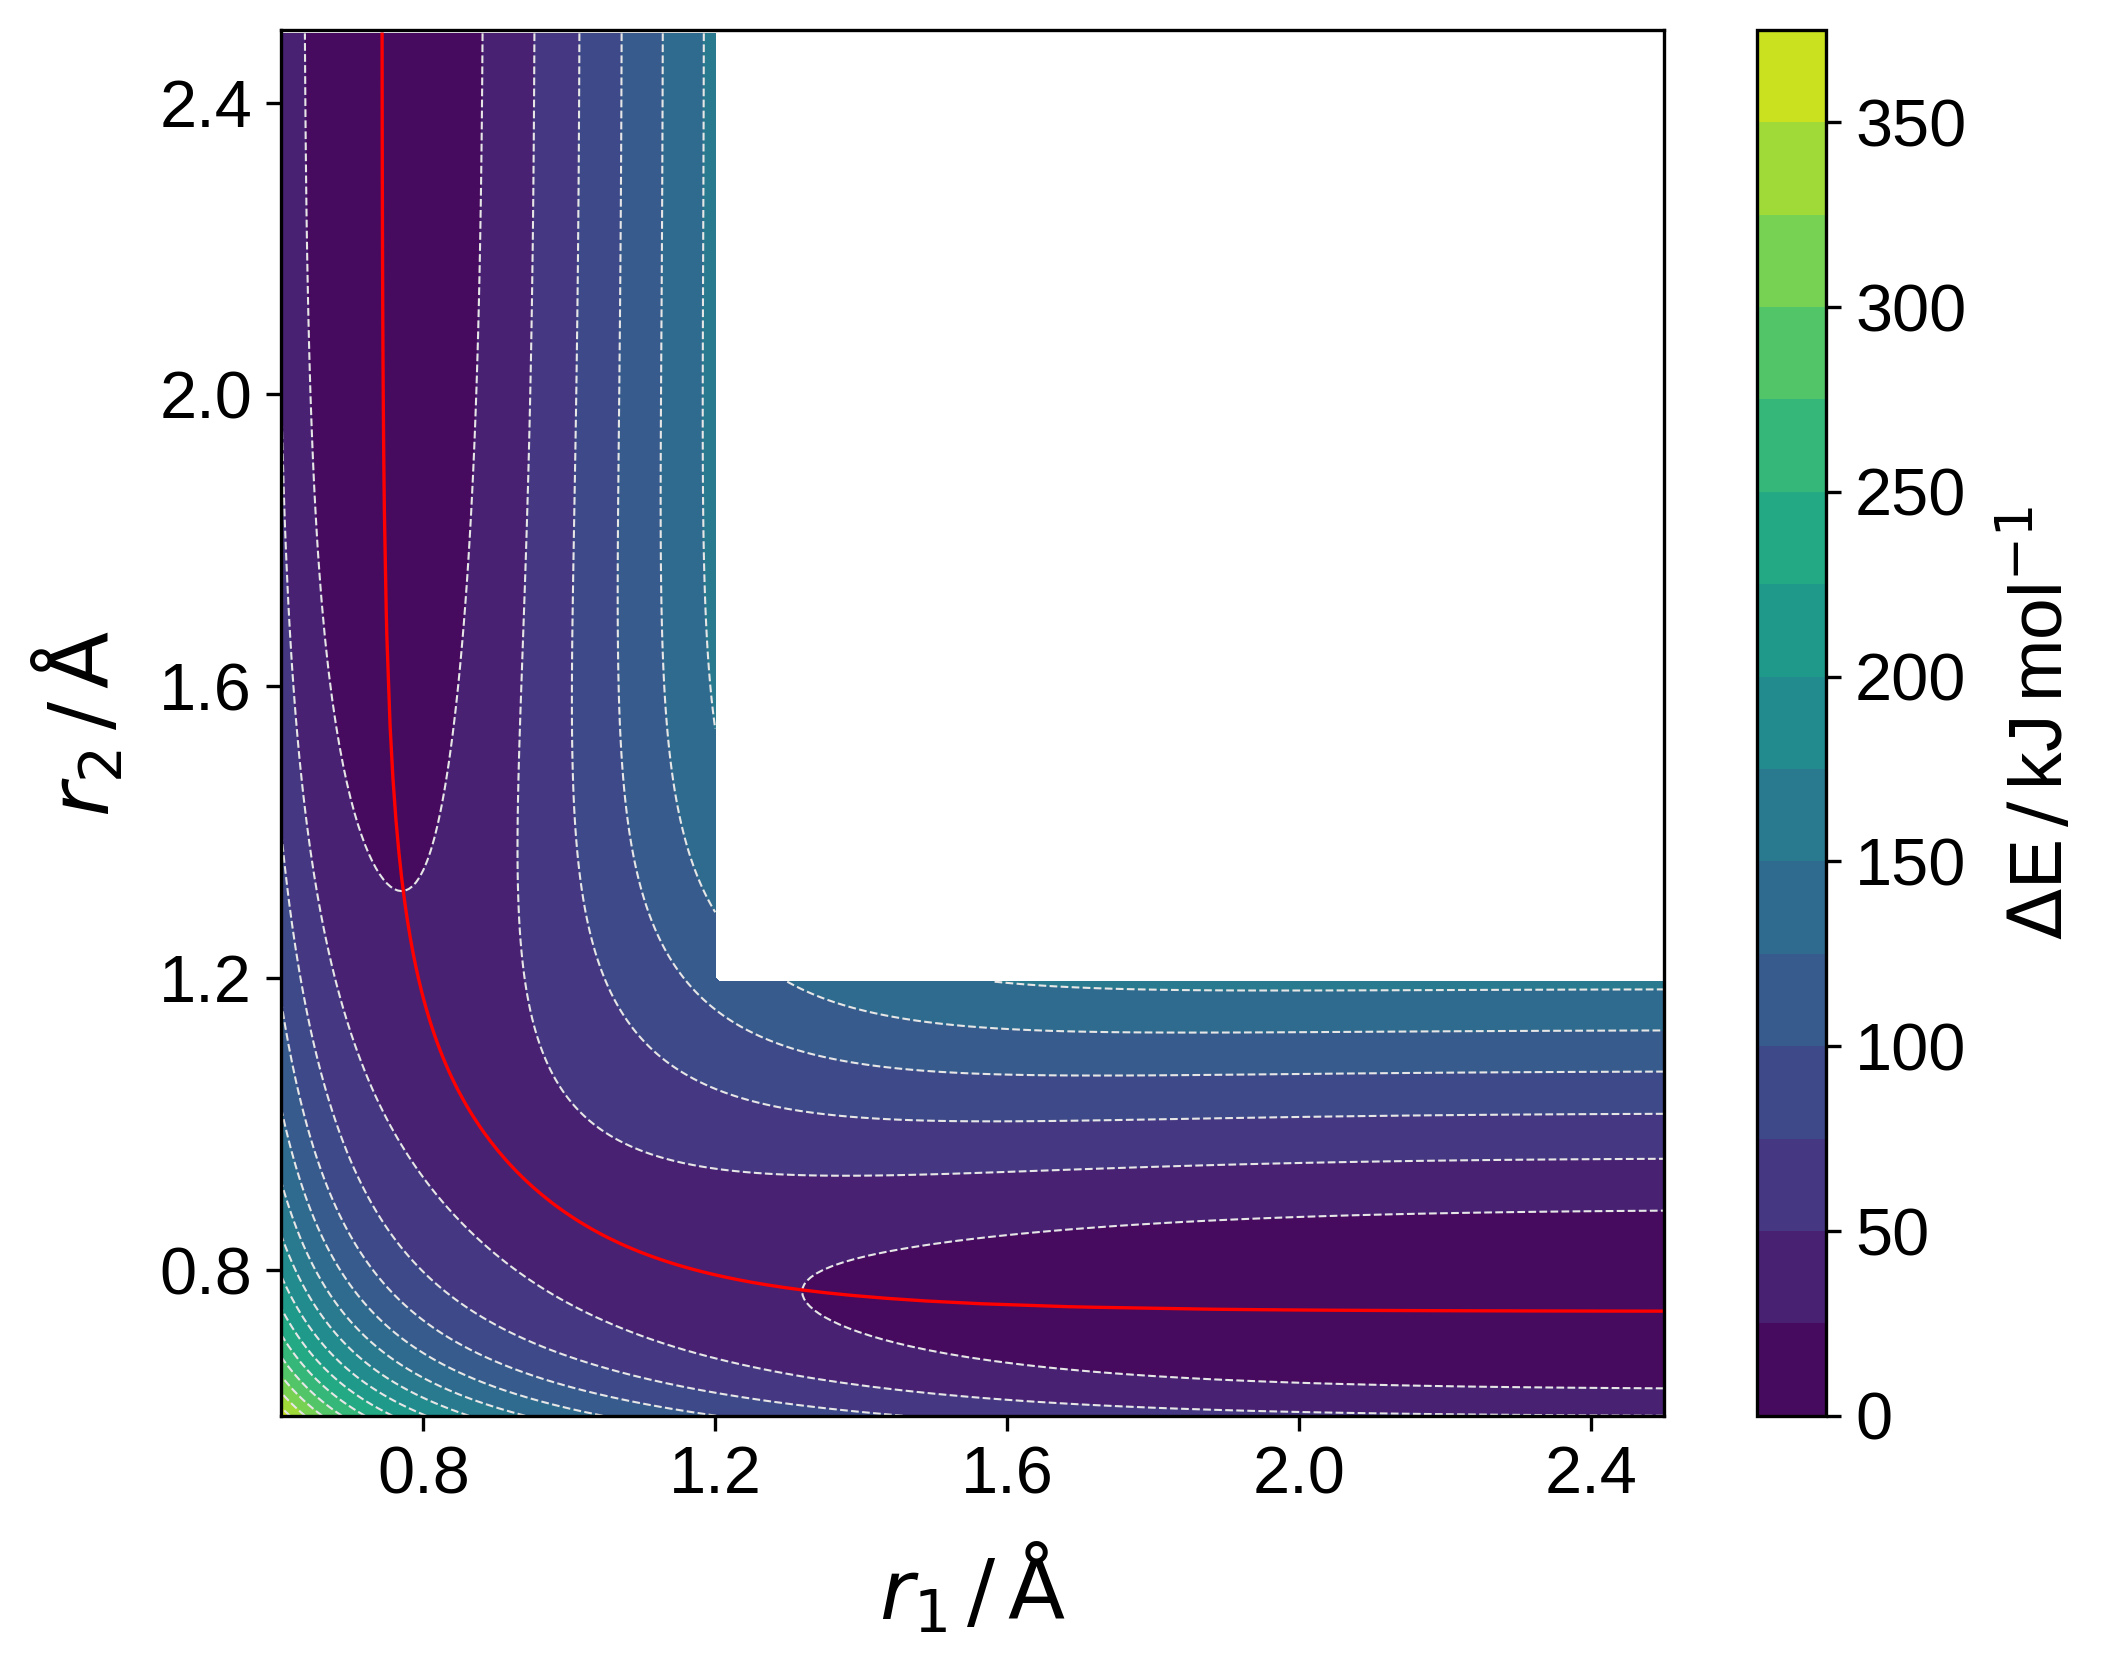
\includegraphics[width=0.62\textwidth]{images/PES_heat_map_ccsd_pertT.png}
\caption{The 2D potential energy surface of the collinear \ce{^2H3} at CCSD(T)/aug-cc-pVTZ}
\end{figure}

\begin{figure}[H]
\centering
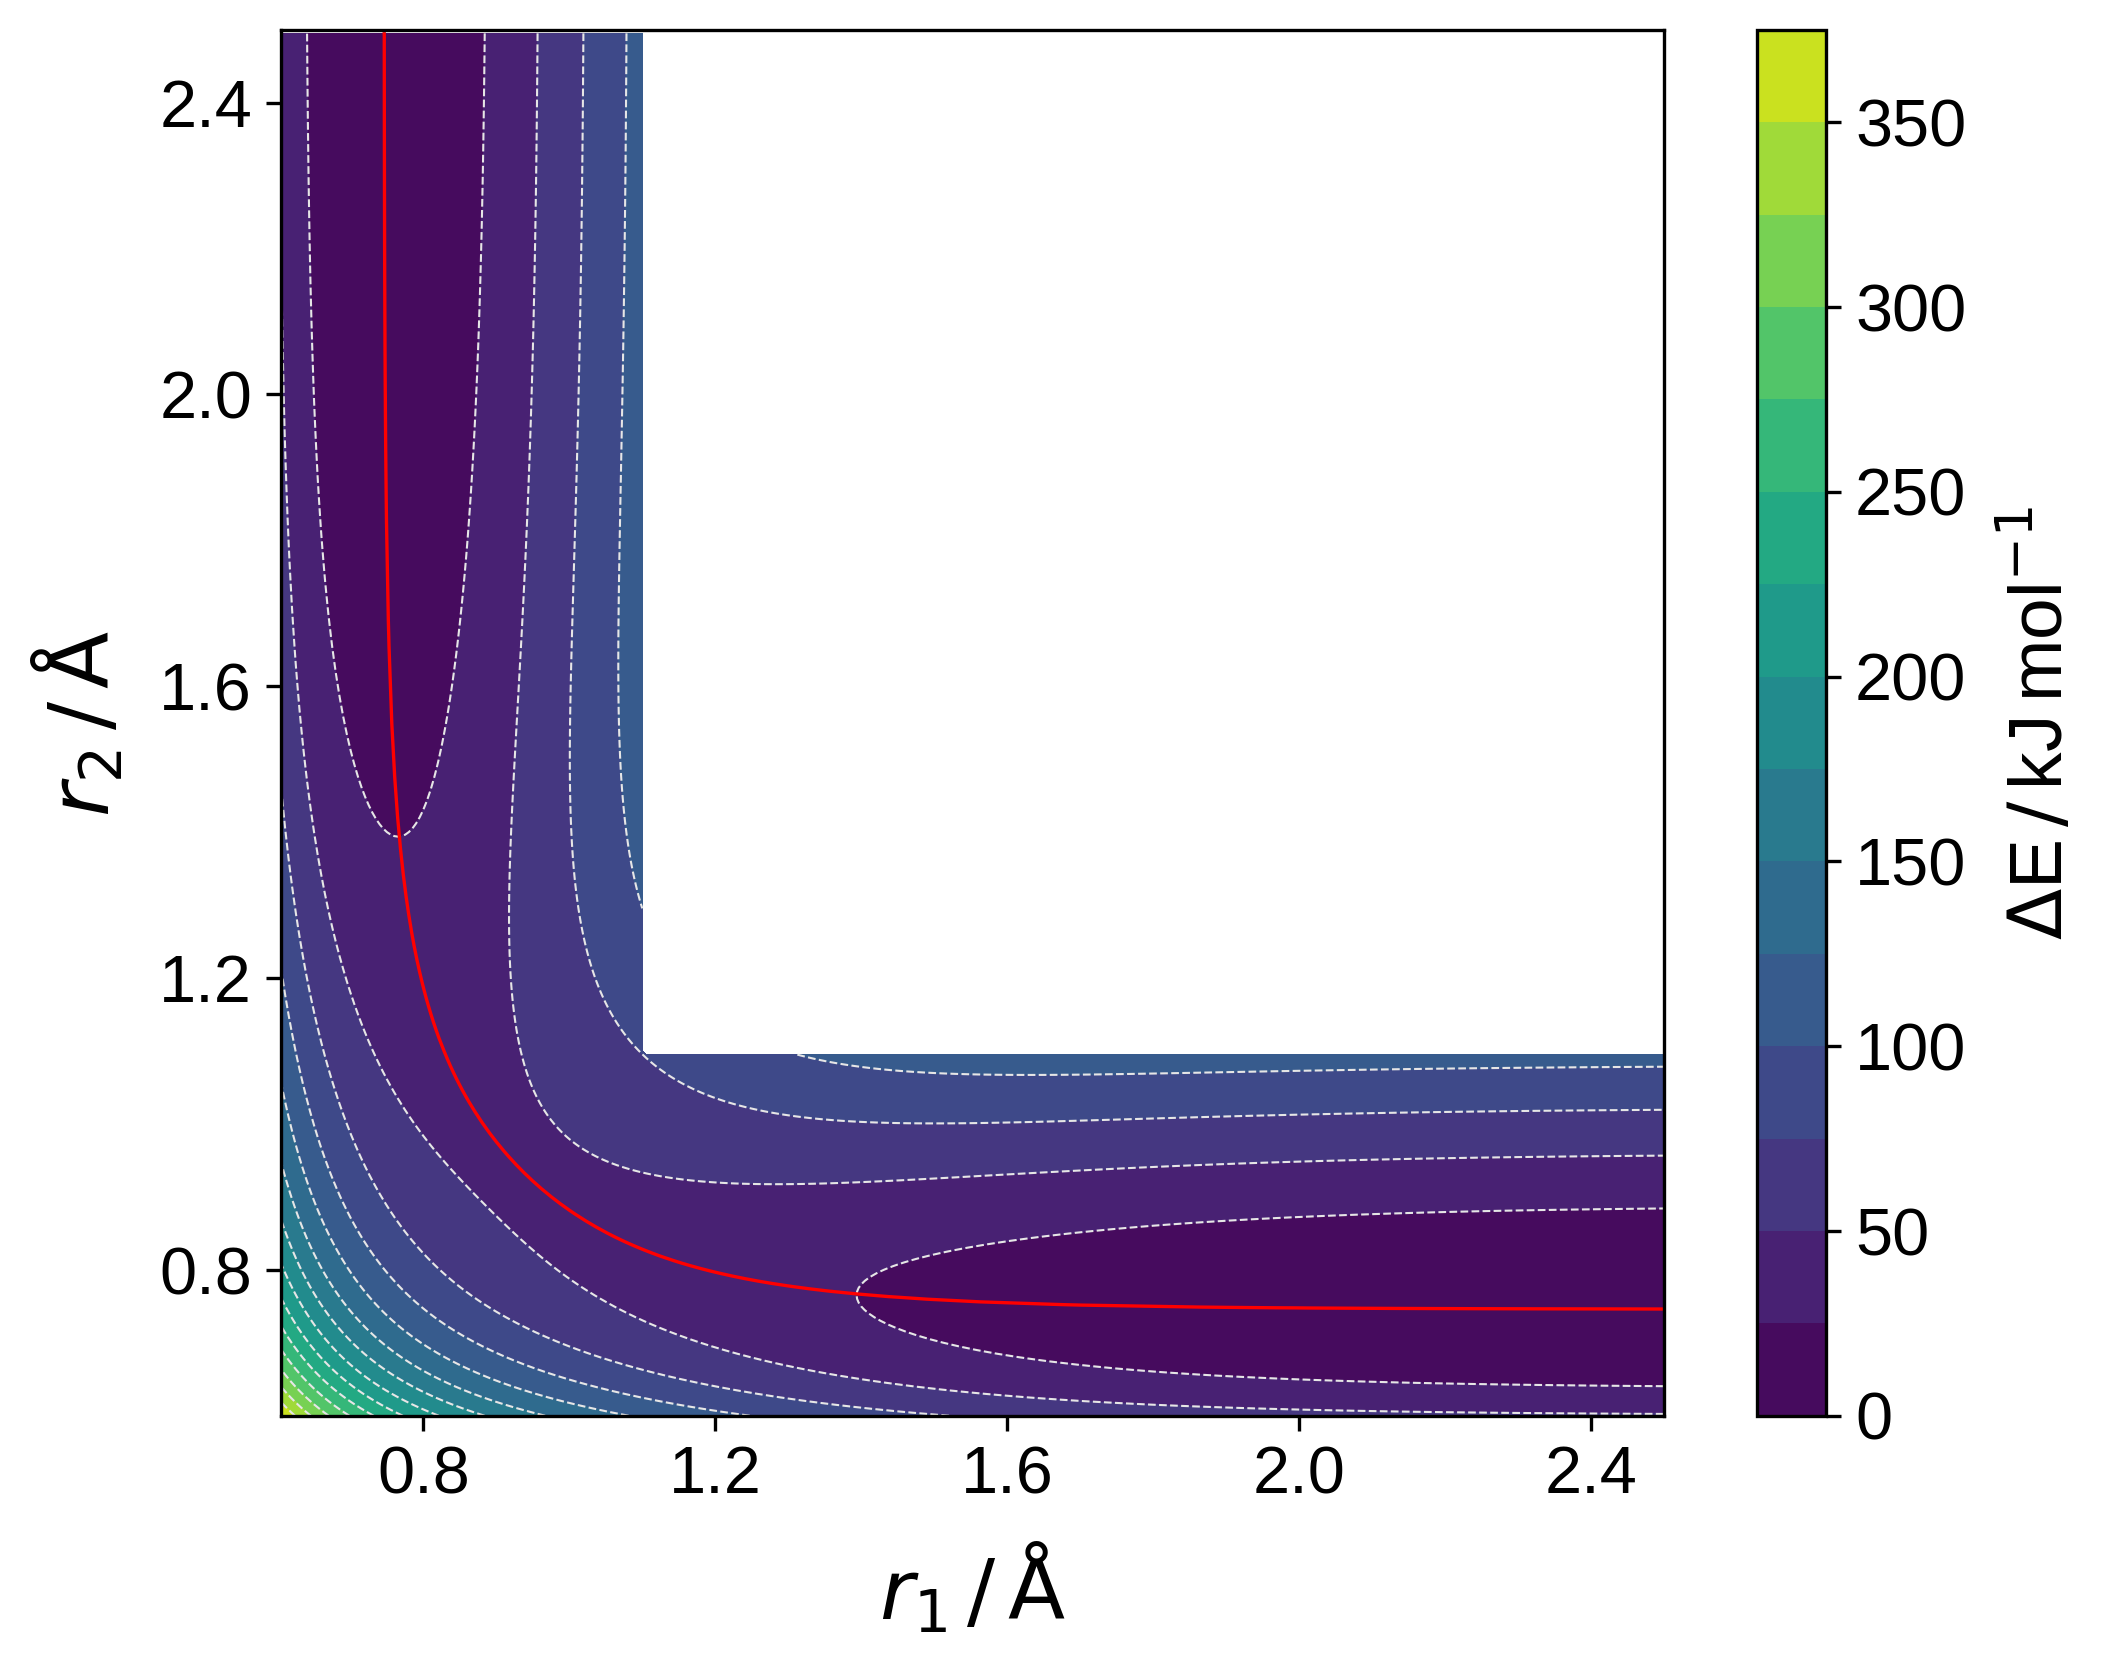
\includegraphics[width=0.62\textwidth]{images/PES_heat_map_ficnevpt2.png}
\caption{The 2D potential energy surface of the collinear \ce{^2H3} at FIC-NEVPT2/aug-cc-pVTZ (CAS 3,3)}
\end{figure}

\section{Doublet (\ce{^2H3}) minimum energy path as singlet (\ce{^1H3+}) and triplet (\ce{^3H3+}): the effects of orbital relaxation}

CASCI with non-optimized natural orbitals (NONOs) was used for the calculation of \ce{^1H3+} singlet and \ce{^3H3+} triplet. We have generated the singlet and triplet states by removing an electron from the doublet system along the MEP. The respective orbitals of the doublet MEP are passed onto the CASCI calculation without performing SCF iterations. Since the natural orbitals of the doublet system were used without optimization in the CASCI ionized states, we have introduced the term pre-ionization natural orbitals (PINOs). These orbitals and the broken bond orbitals (BBOs) can be generally regarded as non-optimized natural orbitals (NONOs) used in CASCI. The PINO orbitals are orthogonal and non-singular transformations were not necessary before CASCI calculations. The kinetic energy from relaxed orbitals of singlet and triplet states contain modulations from orbital relaxation and this prevents identification of electron (de)localization effects solely from Pauli exclusion.\cite{sterling2024} The kinetic energy analysis employed here allows for an explanation of the interactions that take place locally in the bond breaking/making region of a barrier-crossing reaction. As a result, we uncover the important role of Pauli exclusion in the localization of electrons during the barrier-crossing atom exchange of \ce{H2}+\ce{H^.}. The known spin-specific charge transfer\cite{fukui1972} that characterizes the familiar bond-breaking and forming is a manifestation of electron (de)localization that relieves Pauli-exclusion-based localization.

\begin{figure}[H]
\centering
\begin{subfigure}[t]{0.5\textwidth}
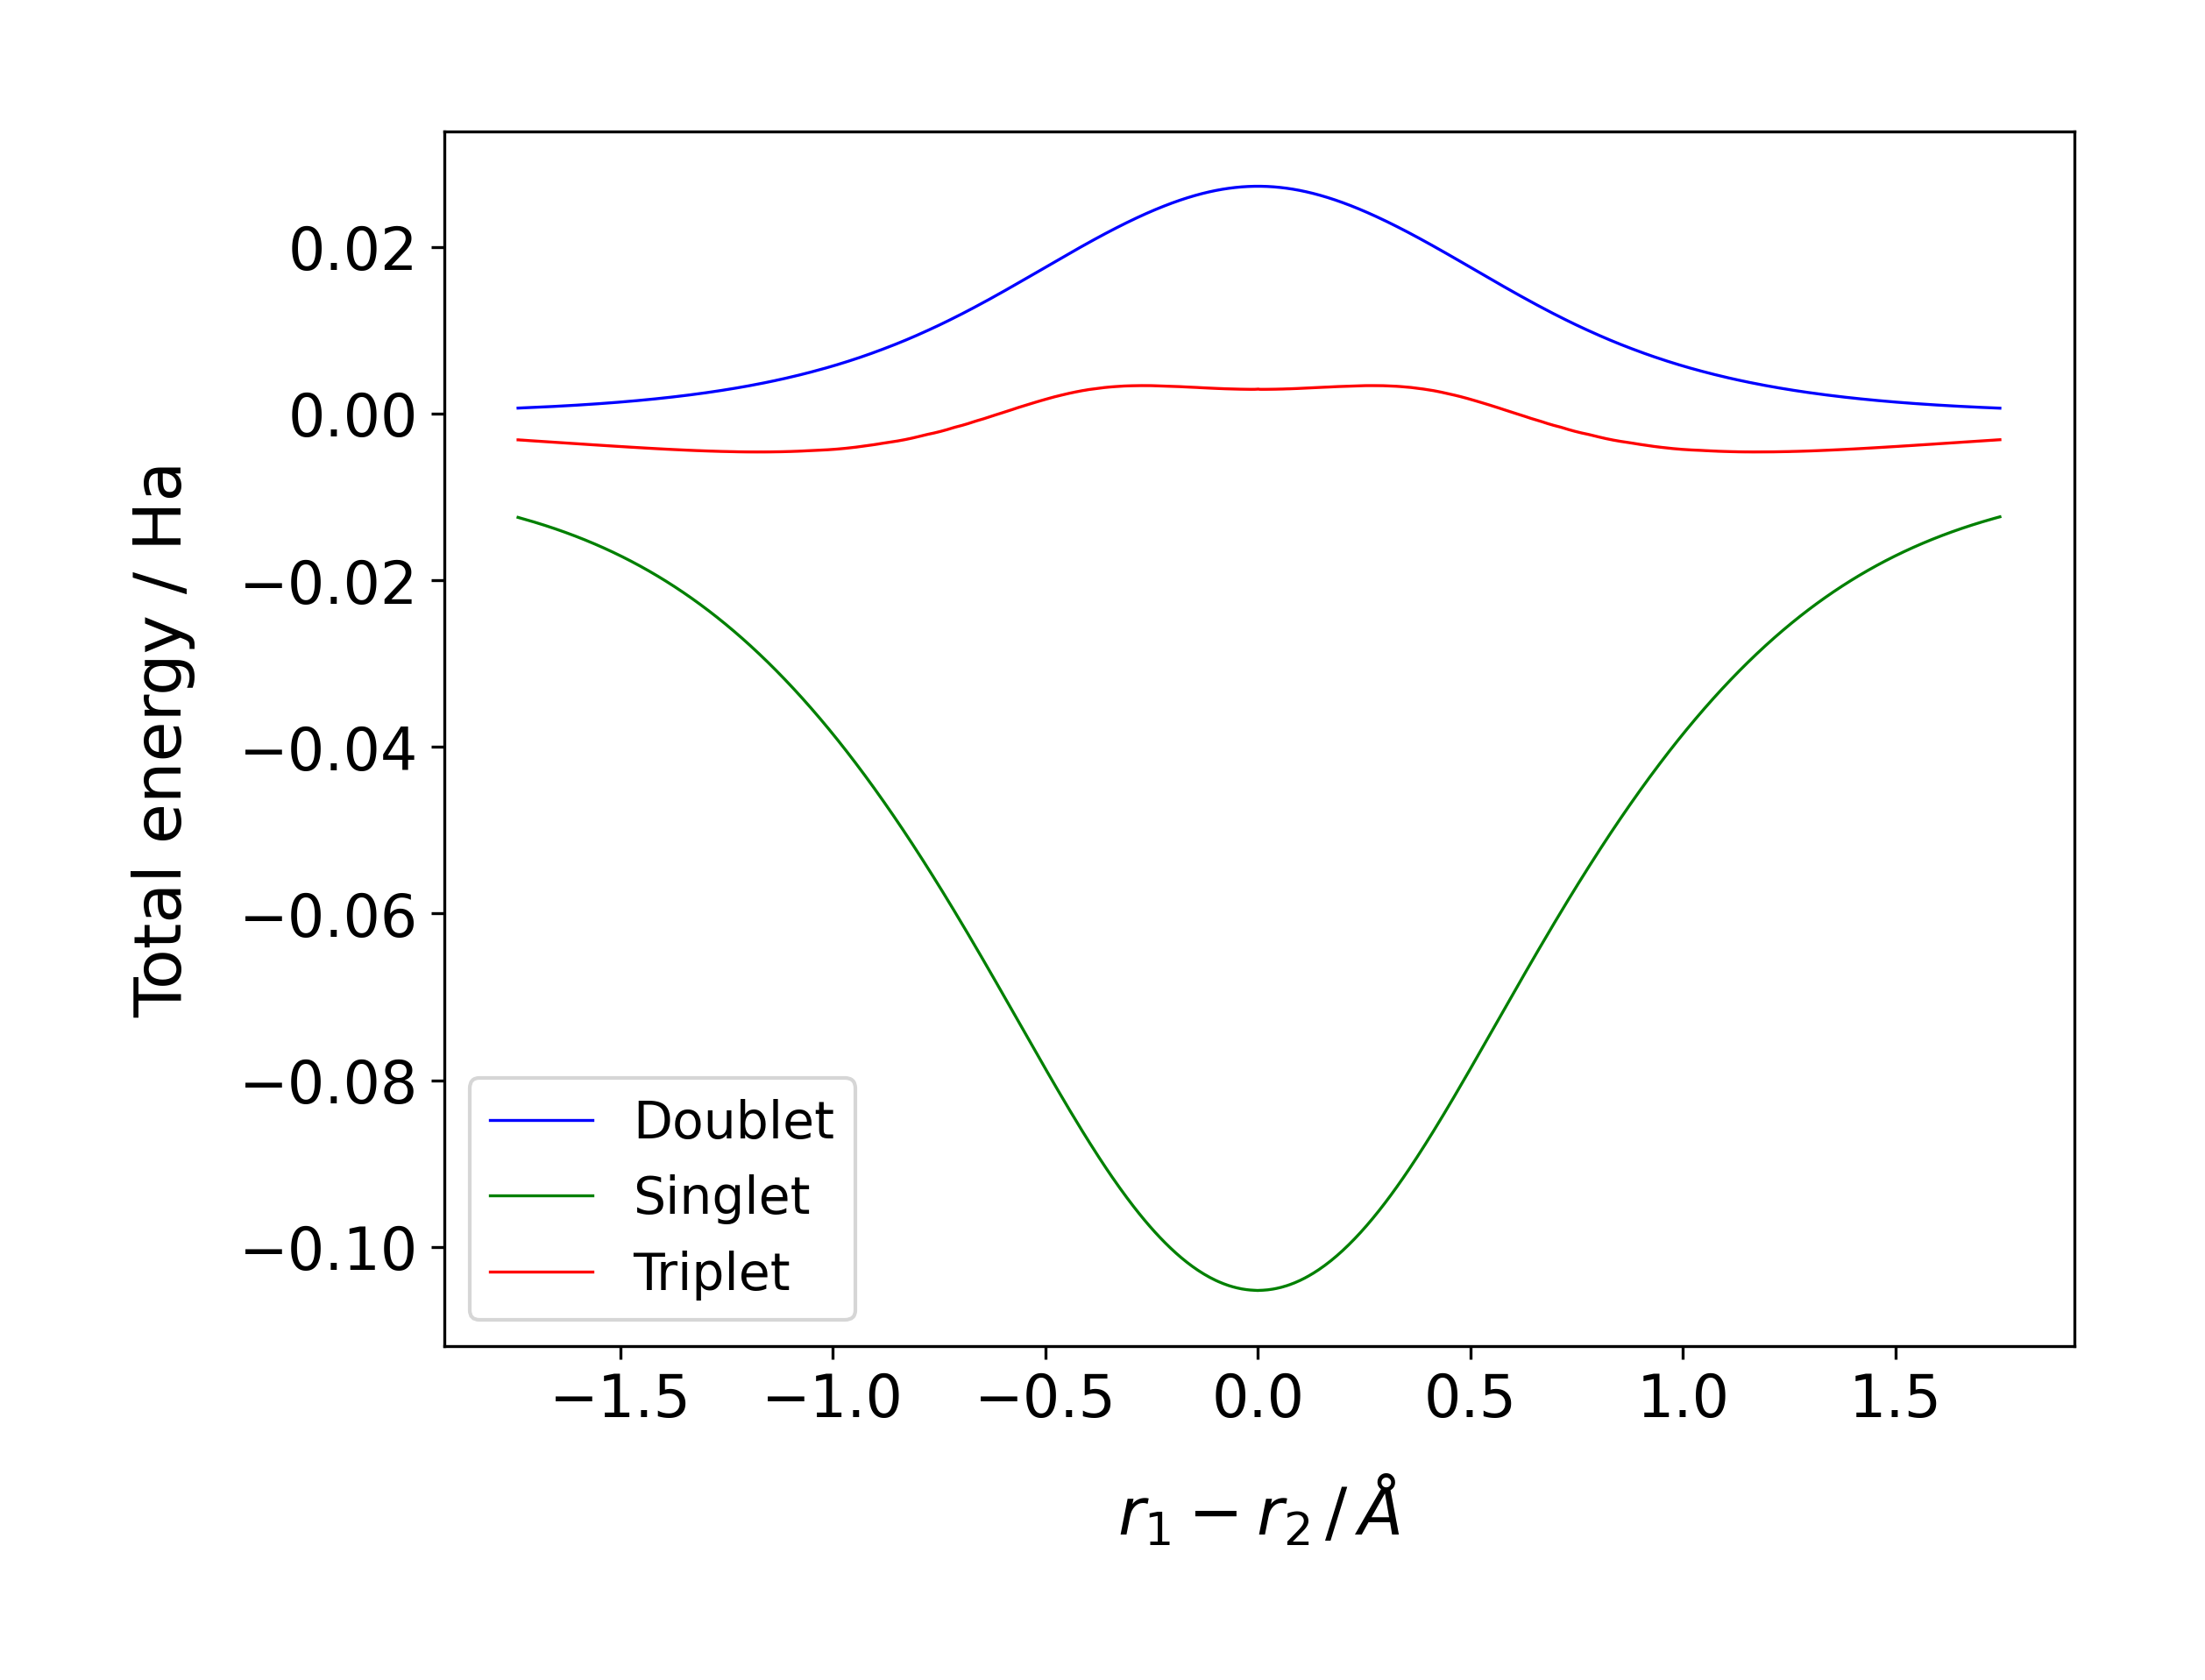
\includegraphics[width=0.9\textwidth]{images/TE_relaxed_normalized_stack.png}
\subcaption{}
\end{subfigure}%
\begin{subfigure}[t]{0.5\textwidth}
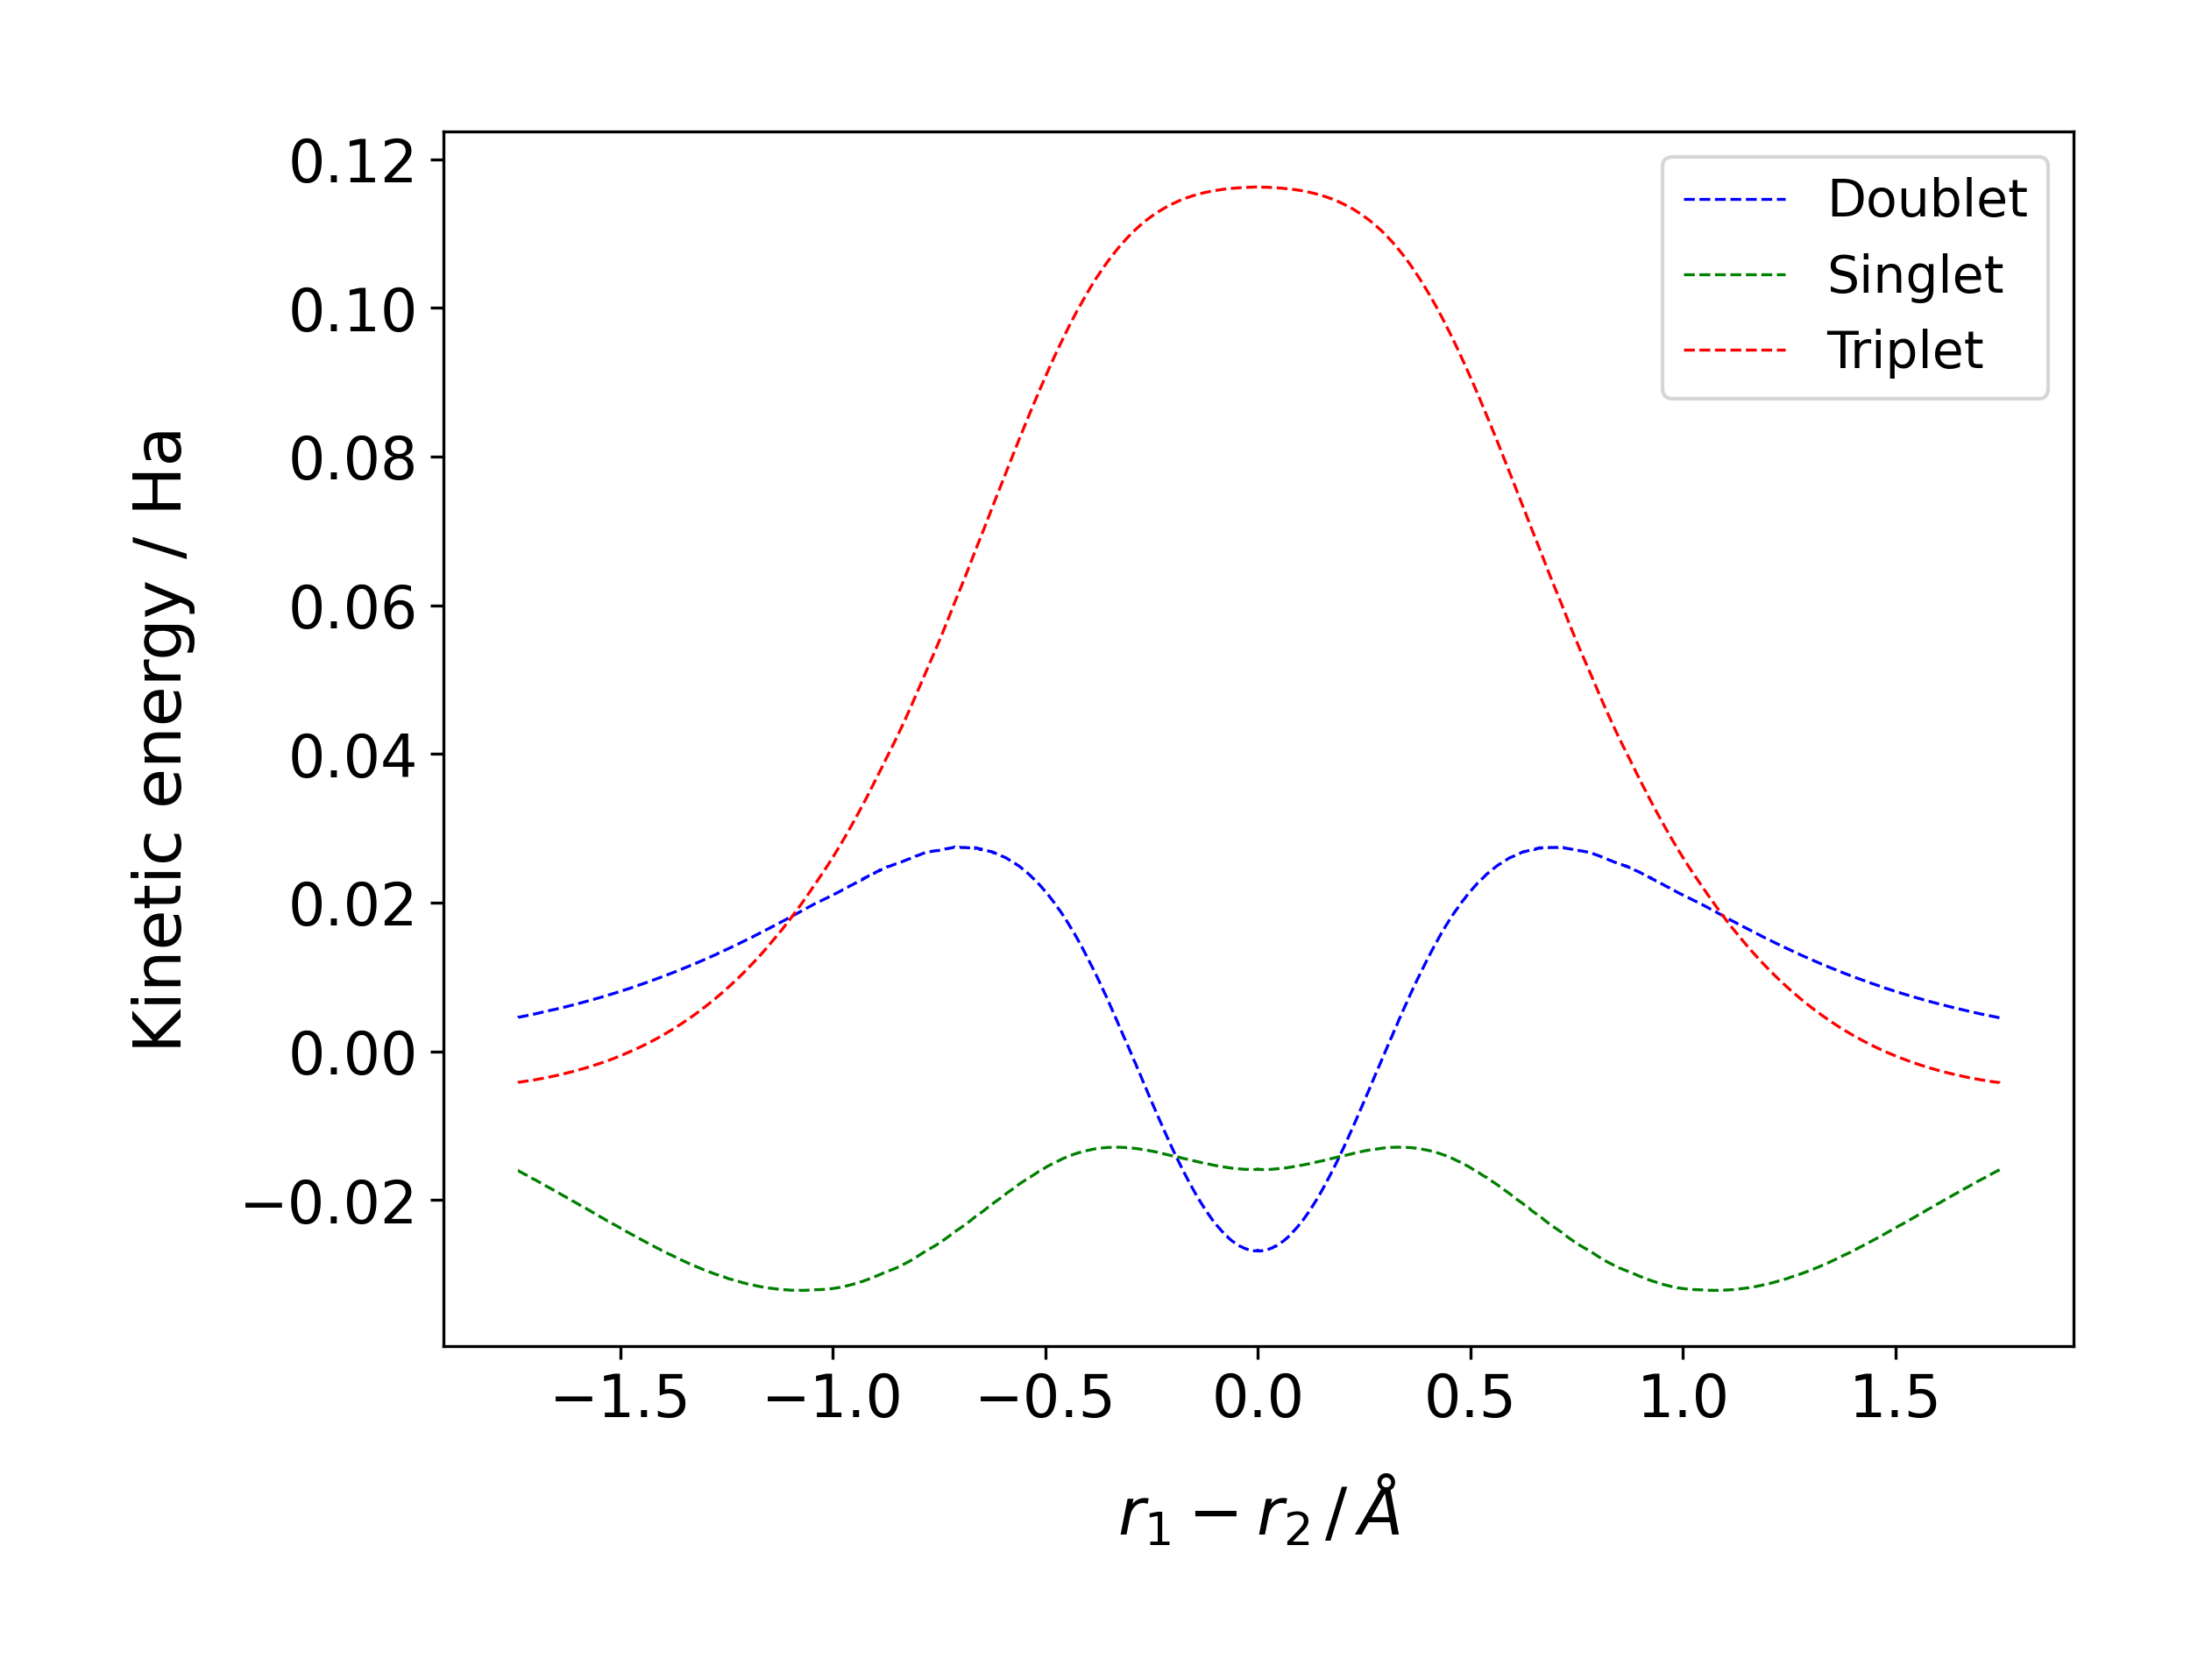
\includegraphics[width=0.9\textwidth]{images/KE_relaxed_normalized_stack.png}
\subcaption{}
\end{subfigure}
\caption{\textbf{(a)} The total energy and \textbf{(b)} the kinetic energy of the orbital relaxed singlet (\ce{^1H3+}) and triplet (\ce{^3H3+}) states of the doublet (\ce{^2H3}) minimum energy path overlaid with the doublet (\ce{^2H3}) energy surfaces}
\end{figure}



\section{Doublet (\ce{^2H3}) kinetic energy derived from the virial theorem}

The kinetic energy of CCSDT and NEVPT2 methods are not directly available. Thus, the virial theorem is used to calculate the kinetic energy from the energy gradients $\left( \frac{\partial E}{\partial R_{\alpha}}\right)$. 

\vspace{0.2in}

\noindent The virial theorem, where $R_{\alpha}$ is the internuclear distance between two nuclei, T is the electronic kinetic energy ($\langle T\rangle$), V is the potential energy ($\langle V\rangle$) and E is the total energy can be written as,
\begin{equation}
2T + V + \sum_{\alpha=1}^NR_{\alpha}\frac{{\partial}E}{{\partial}R_{\alpha}} = 0
\end{equation}

since $T+V=E$

\begin{equation}
T = - \left( E + \sum_{\alpha=1}^NR_{\alpha}\frac{{\partial}E}{{\partial}R_{\alpha}}\right)
\end{equation}

For NEVPT2, numerical gradients are available from the ORCA 6.0.1. However, CCSDT gradients (numerical or analytical) are not available from ORCA 6.0.1 nor Q-Chem 6.2.1. Thus, CCSDT energy gradients are obtained numerically using the single point energies of perturbed \ce{H3} system and the central differences method. Since the \ce{H3} system is aligned in the z-direction of Cartesian space, the perturbations are only required in the z-direction. By choosing the central atom to be the Cartesian origin we can neglect forces on the central atom. Hence, the four perturbations of two outer atoms are considered in positive and negative z-direction for the gradient calculation. The gradient of kinetic energy is obtained using the central differences method and the noisy data is fitted with a spline (make\_smoothing\_spline of SciPy). Spline fitting agrees on points of interest in our kinetic energy analysis and we believe the qualitative information from the fitted splines are sufficient. It was noted the perturbation based calculations give a diminished magnitude of the gradient compared to that of CCSDT and CASSCF.

\begin{figure}[H]
\centering
\begin{subfigure}[t]{0.5\textwidth}
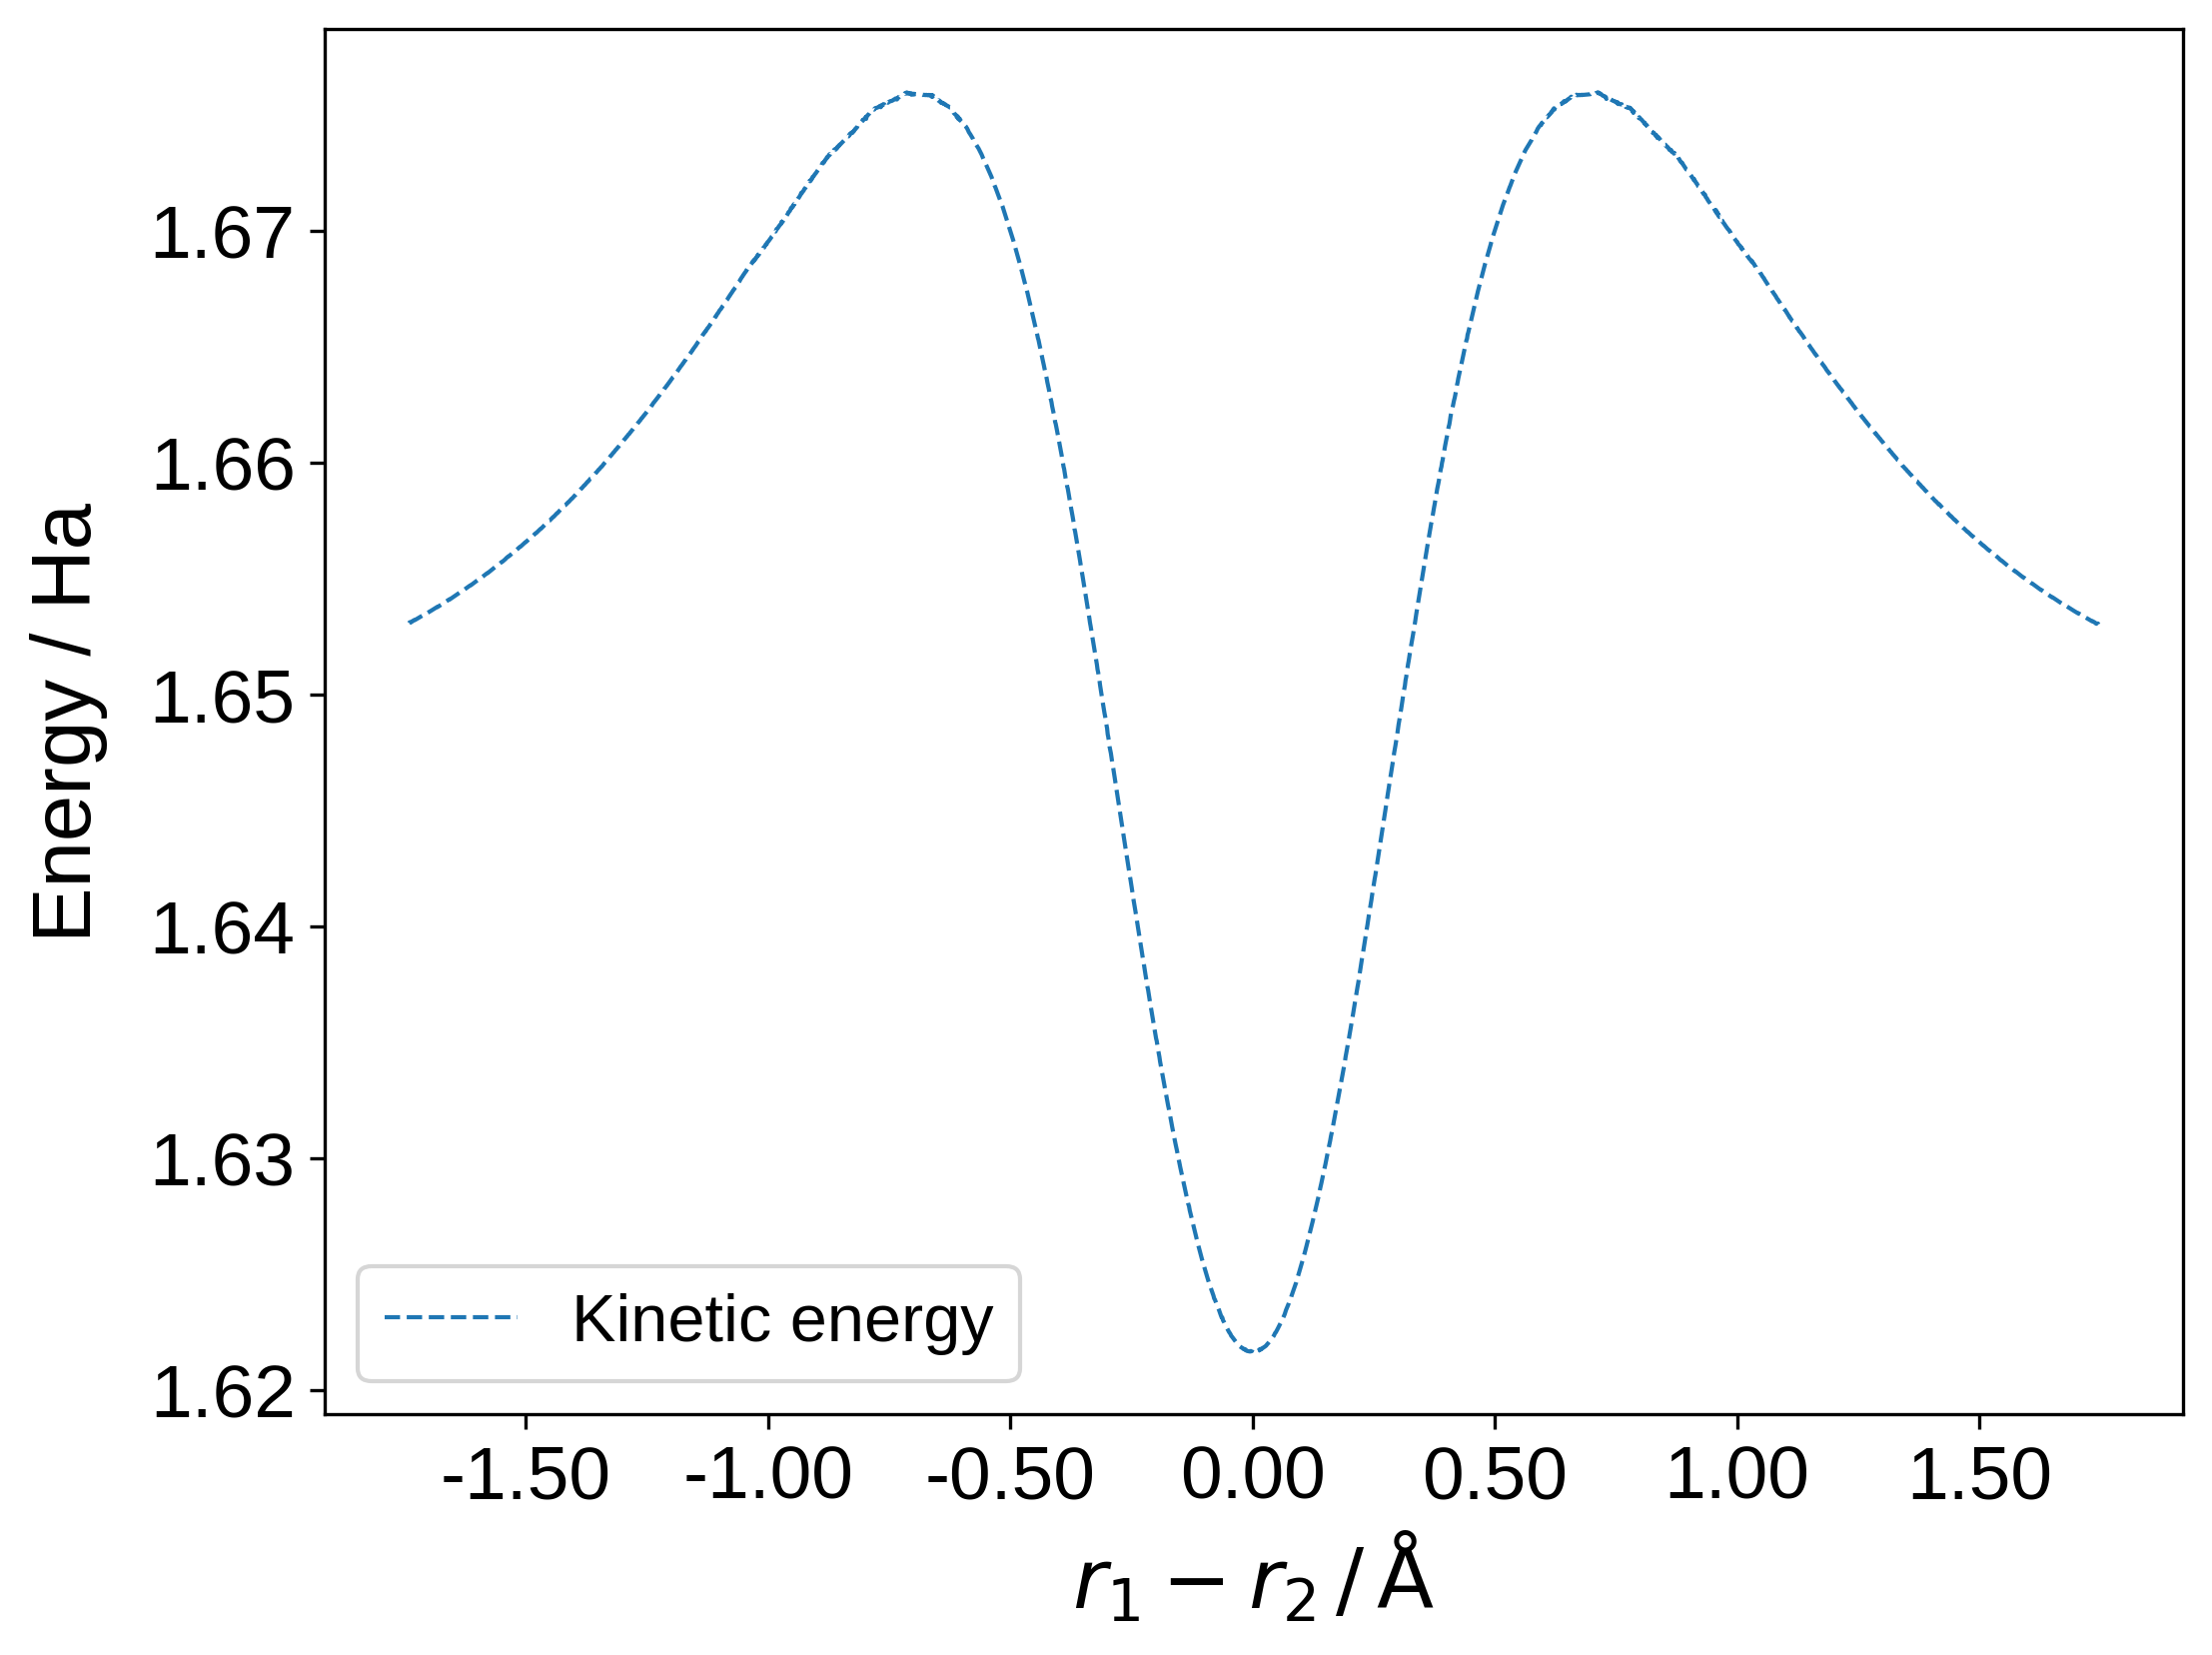
\includegraphics[width=0.9\textwidth]{images/CASSCF_KE.png}
\subcaption{}
\end{subfigure}%
\begin{subfigure}[t]{0.5\textwidth}
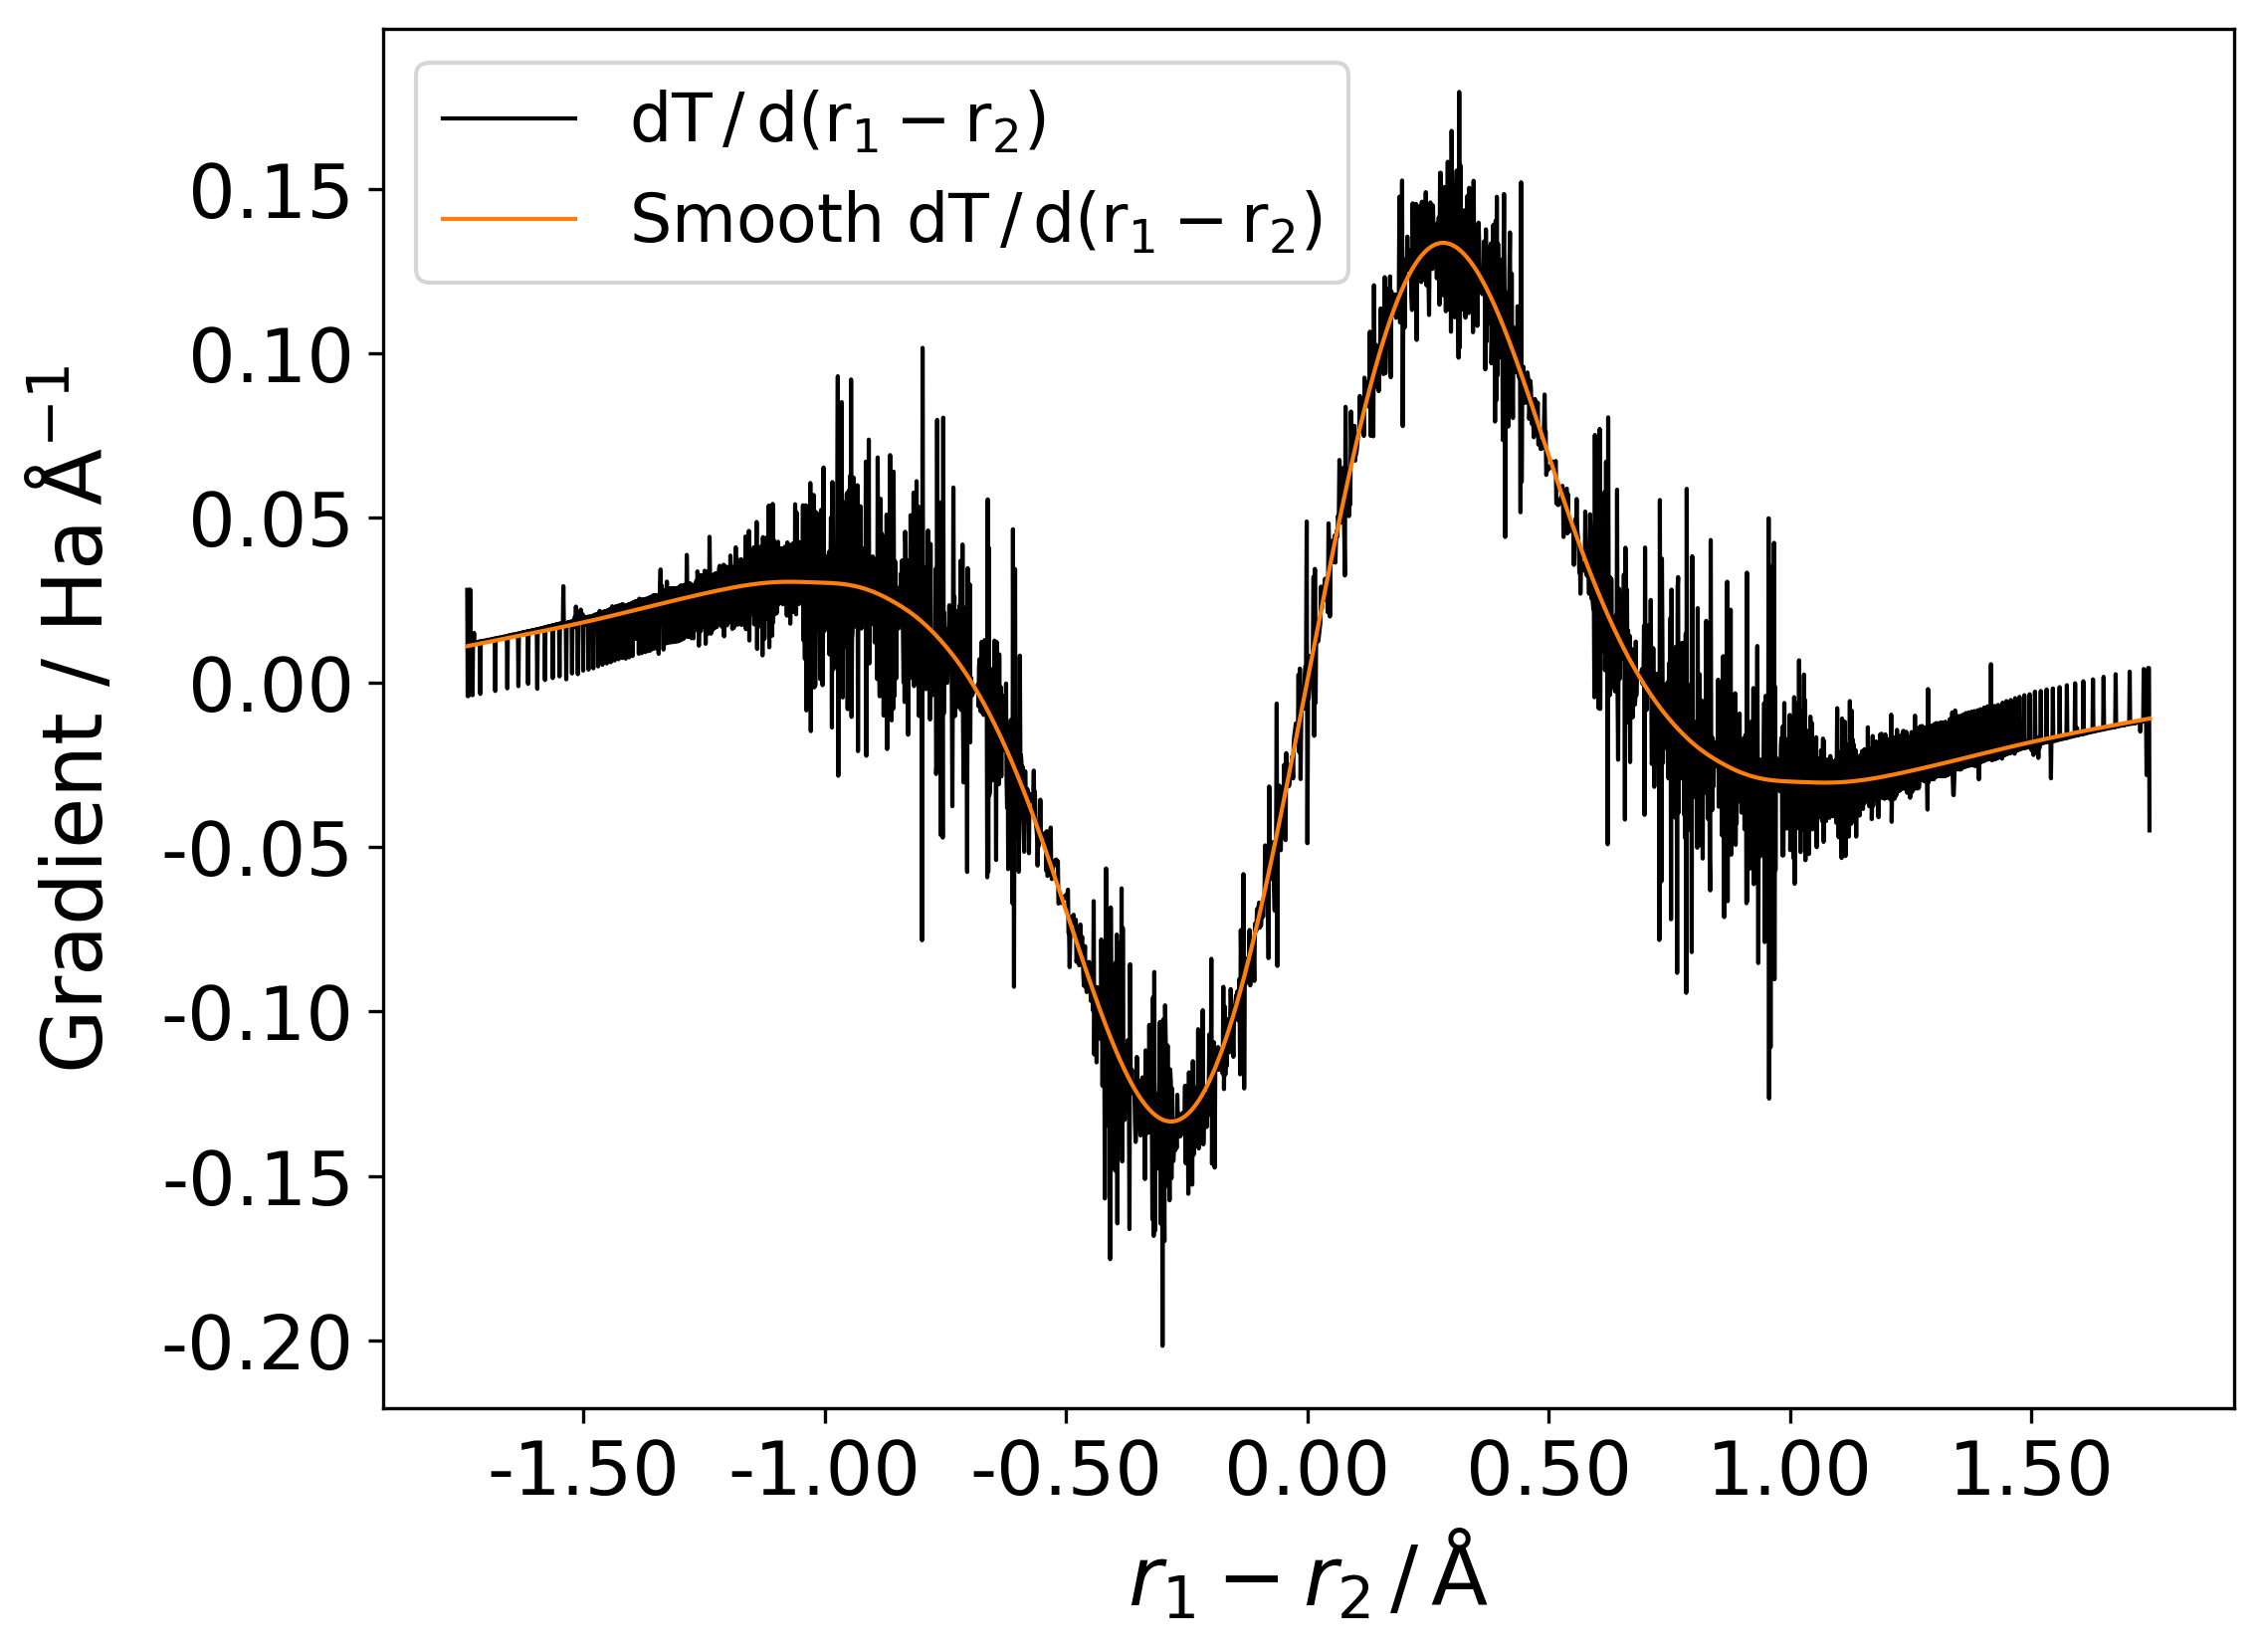
\includegraphics[width=0.9\textwidth]{images/CASSCF_KE_grad.png}
\subcaption{}
\end{subfigure}
\caption{\textbf{(a)} CASSCF/aug-cc-pVTZ  kinetic energy calculated from the wavefunction, \textbf{(b)} gradient of the kinetic energy and the fitted spline}
\end{figure}

\begin{figure}[H]
\centering
\begin{subfigure}[t]{0.5\textwidth}
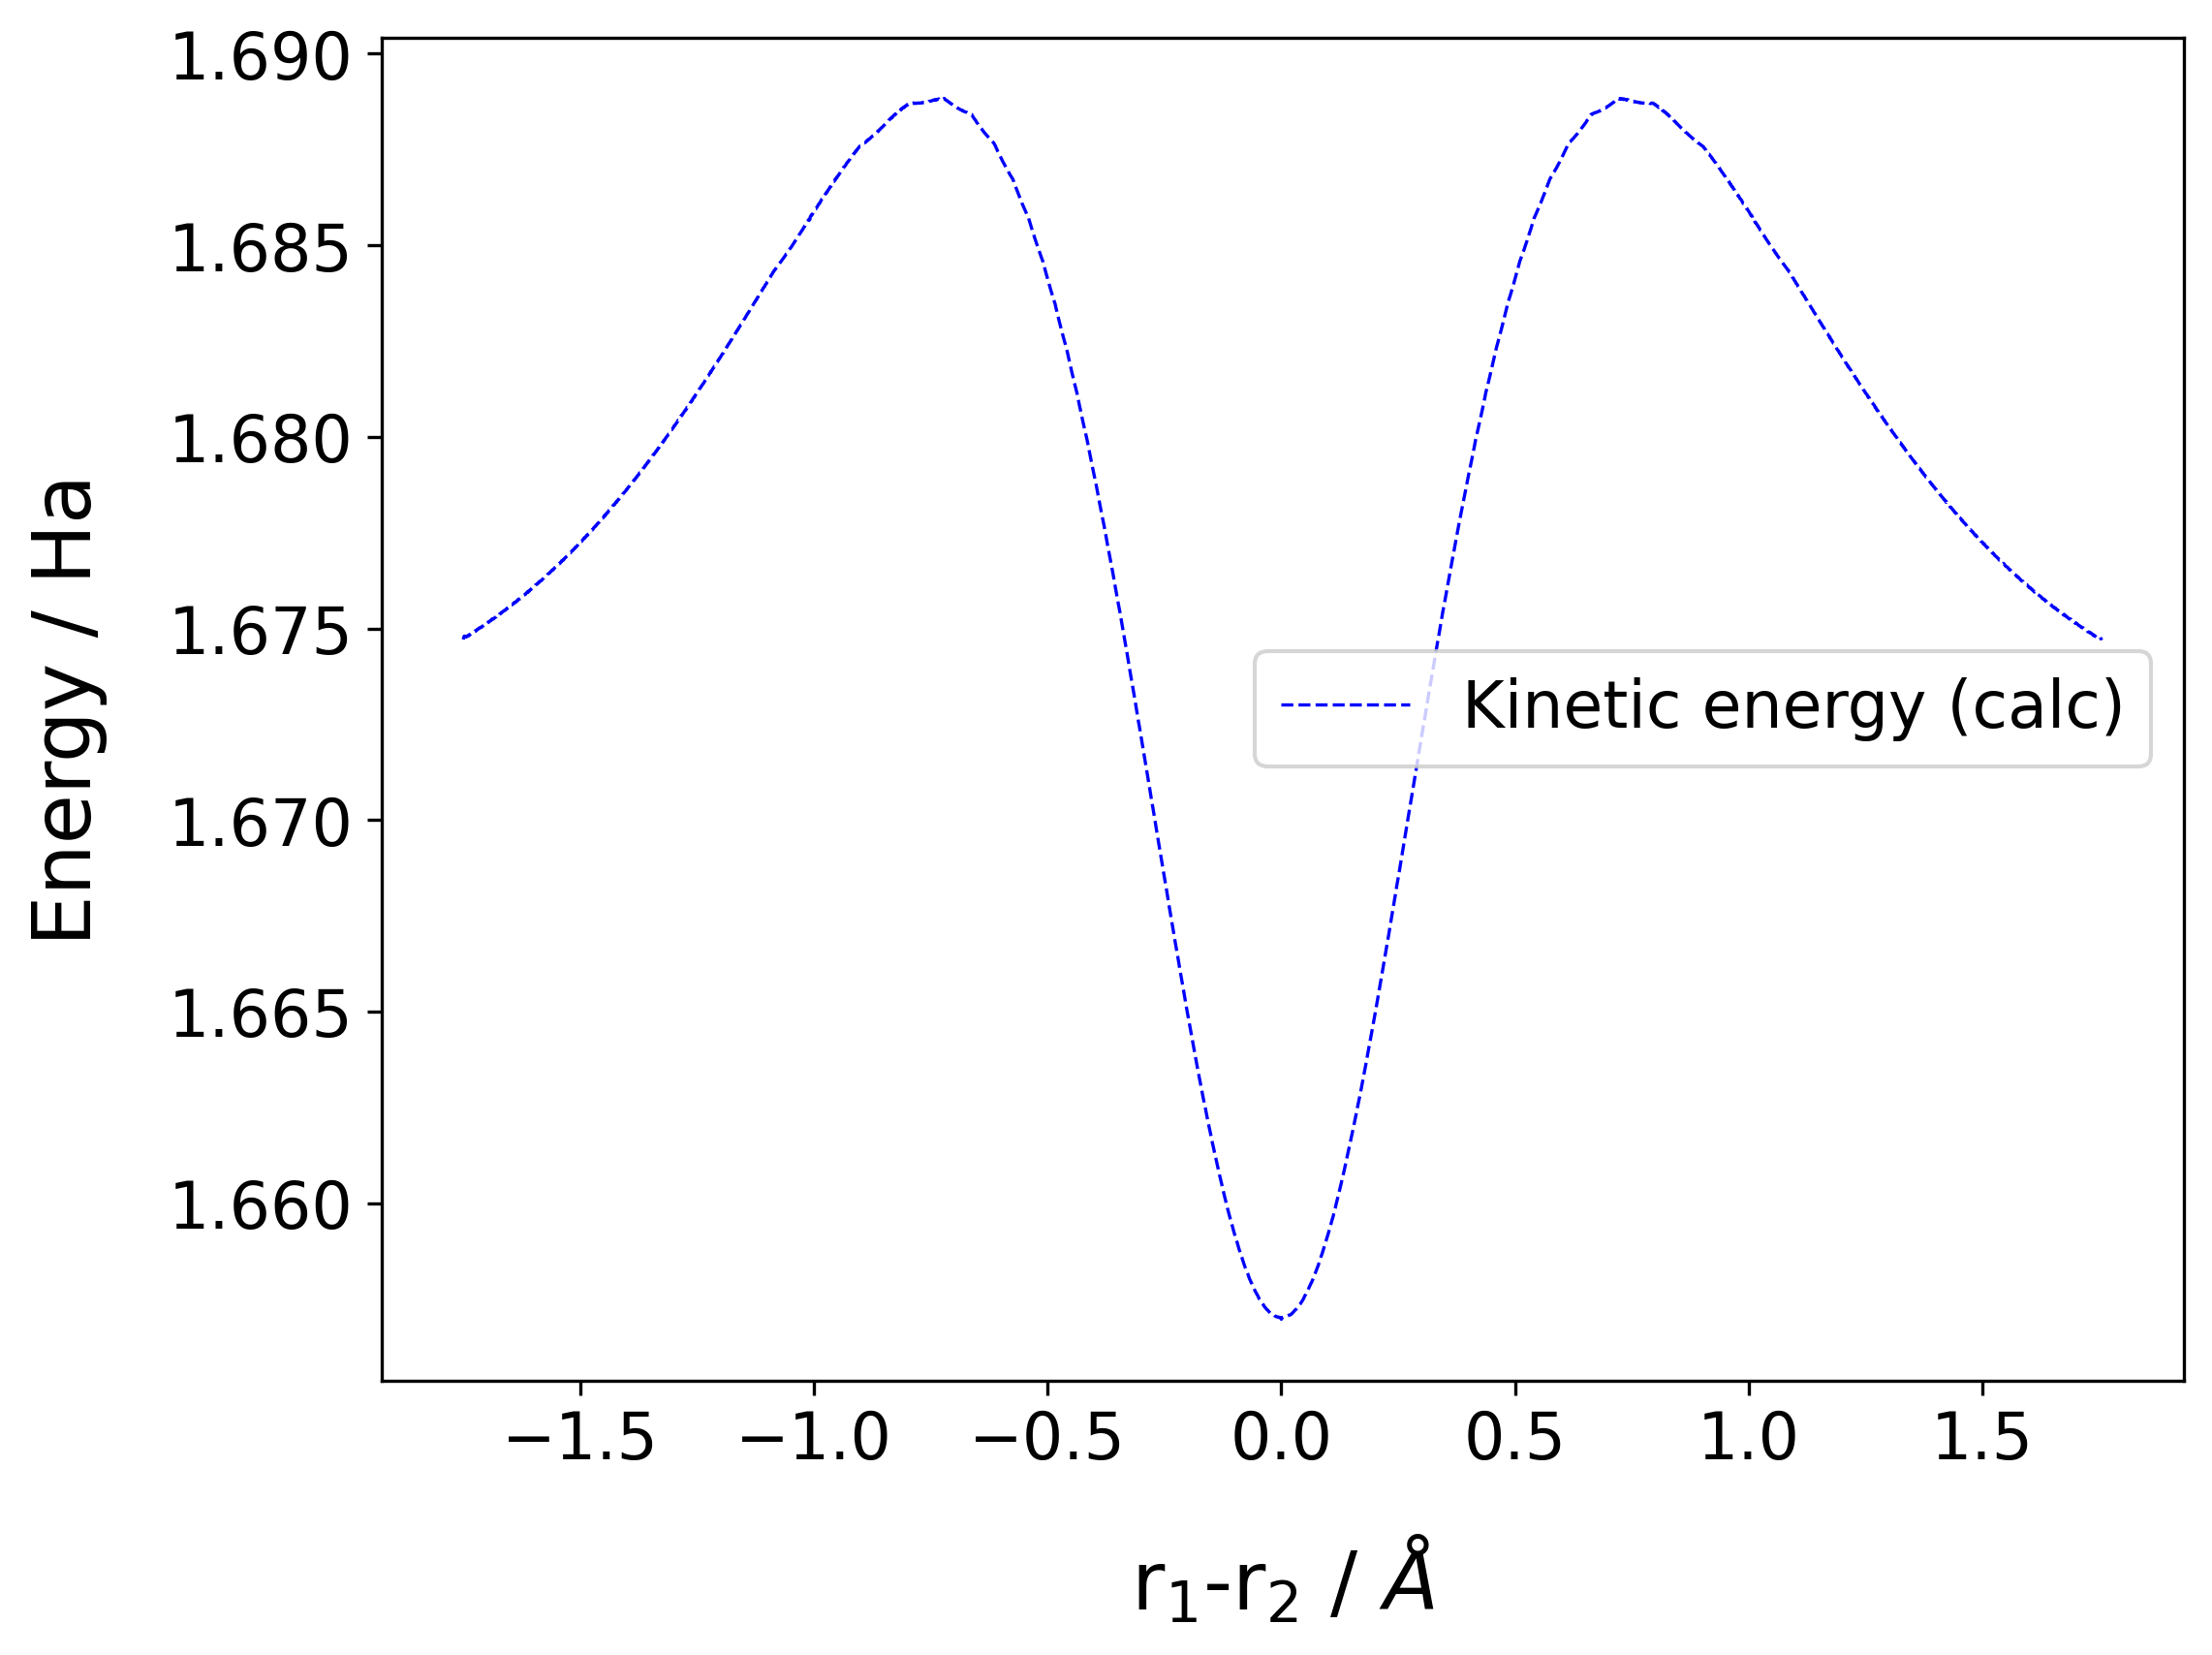
\includegraphics[width=0.9\textwidth]{images/ccsdt_KE.png}
\subcaption{}
\end{subfigure}%
\begin{subfigure}[t]{0.5\textwidth}
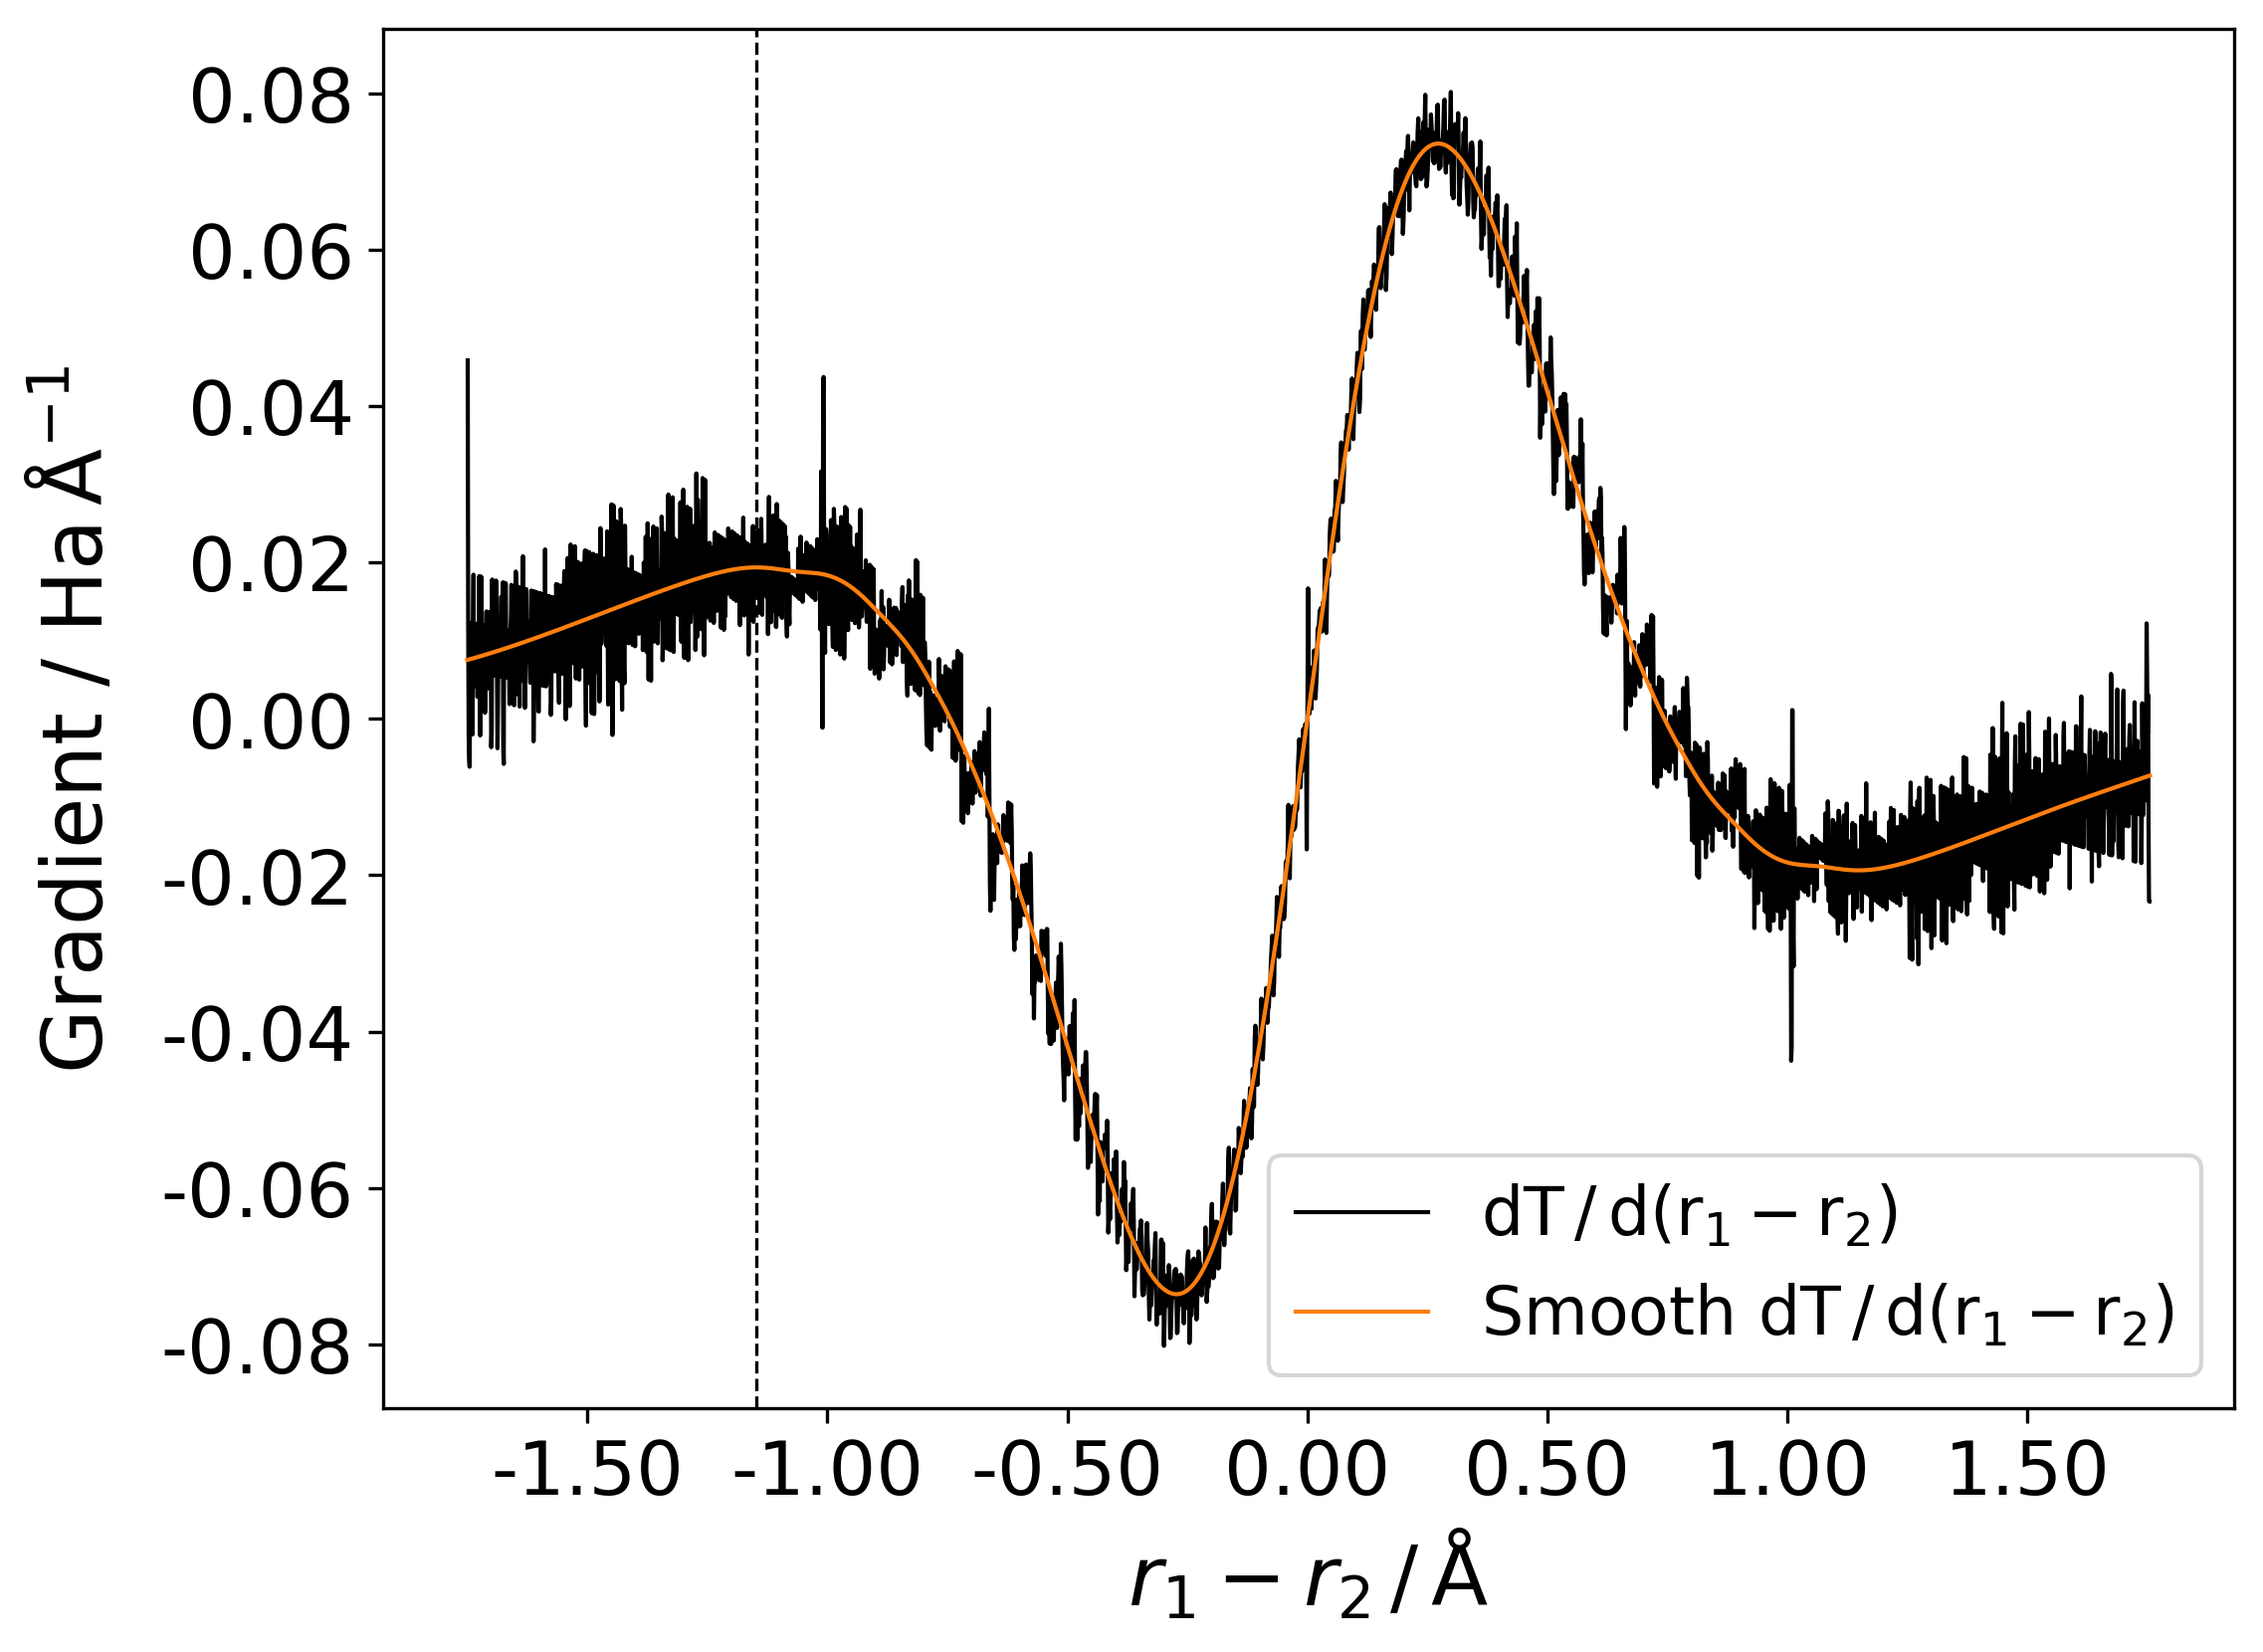
\includegraphics[width=0.9\textwidth]{images/ccsdt_KE_grad.png}
\subcaption{}
\end{subfigure}
\caption{\textbf{(a)} CCSDT/aug-cc-pVTZ kinetic energy calculated from the numerical energy gradient and virial theorem, \textbf{(b)} gradient of the kinetic energy and the fitted spline}
\end{figure}

\begin{figure}[H]
\centering
\begin{subfigure}[t]{0.5\textwidth}
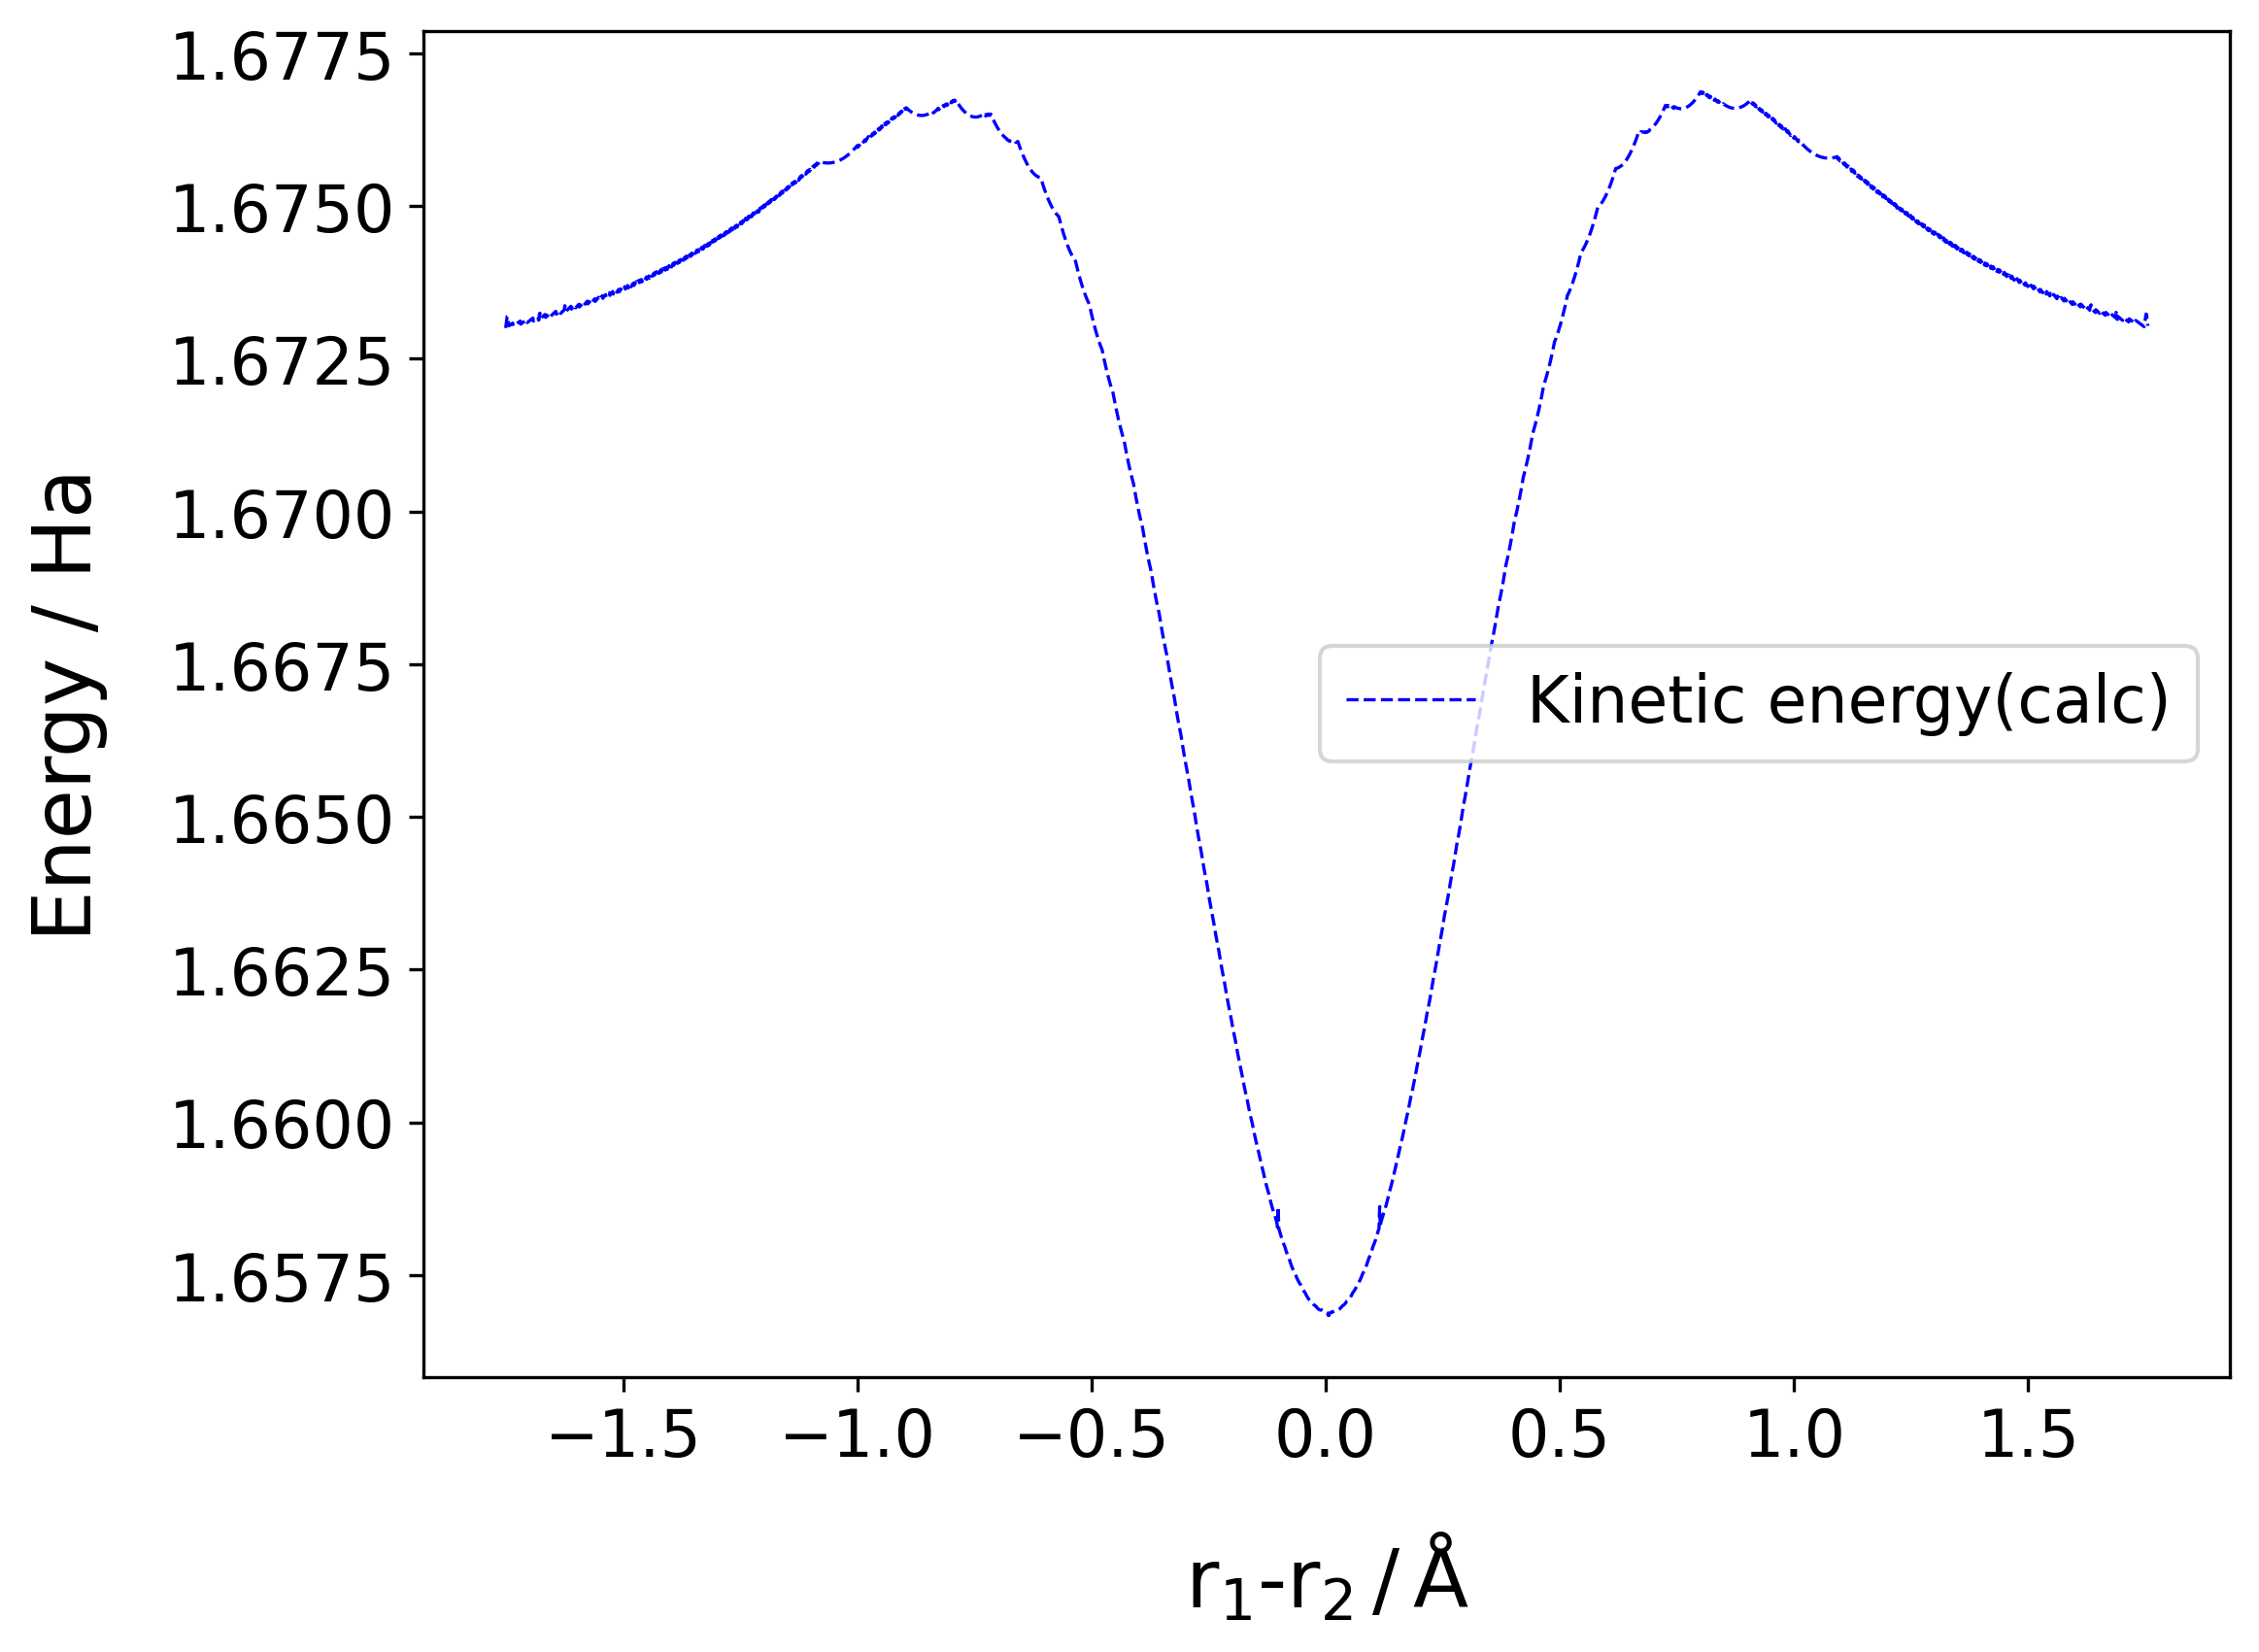
\includegraphics[width=0.9\textwidth]{images/ccsd_pertT_KE.png}
\subcaption{}
\end{subfigure}%
\begin{subfigure}[t]{0.5\textwidth}
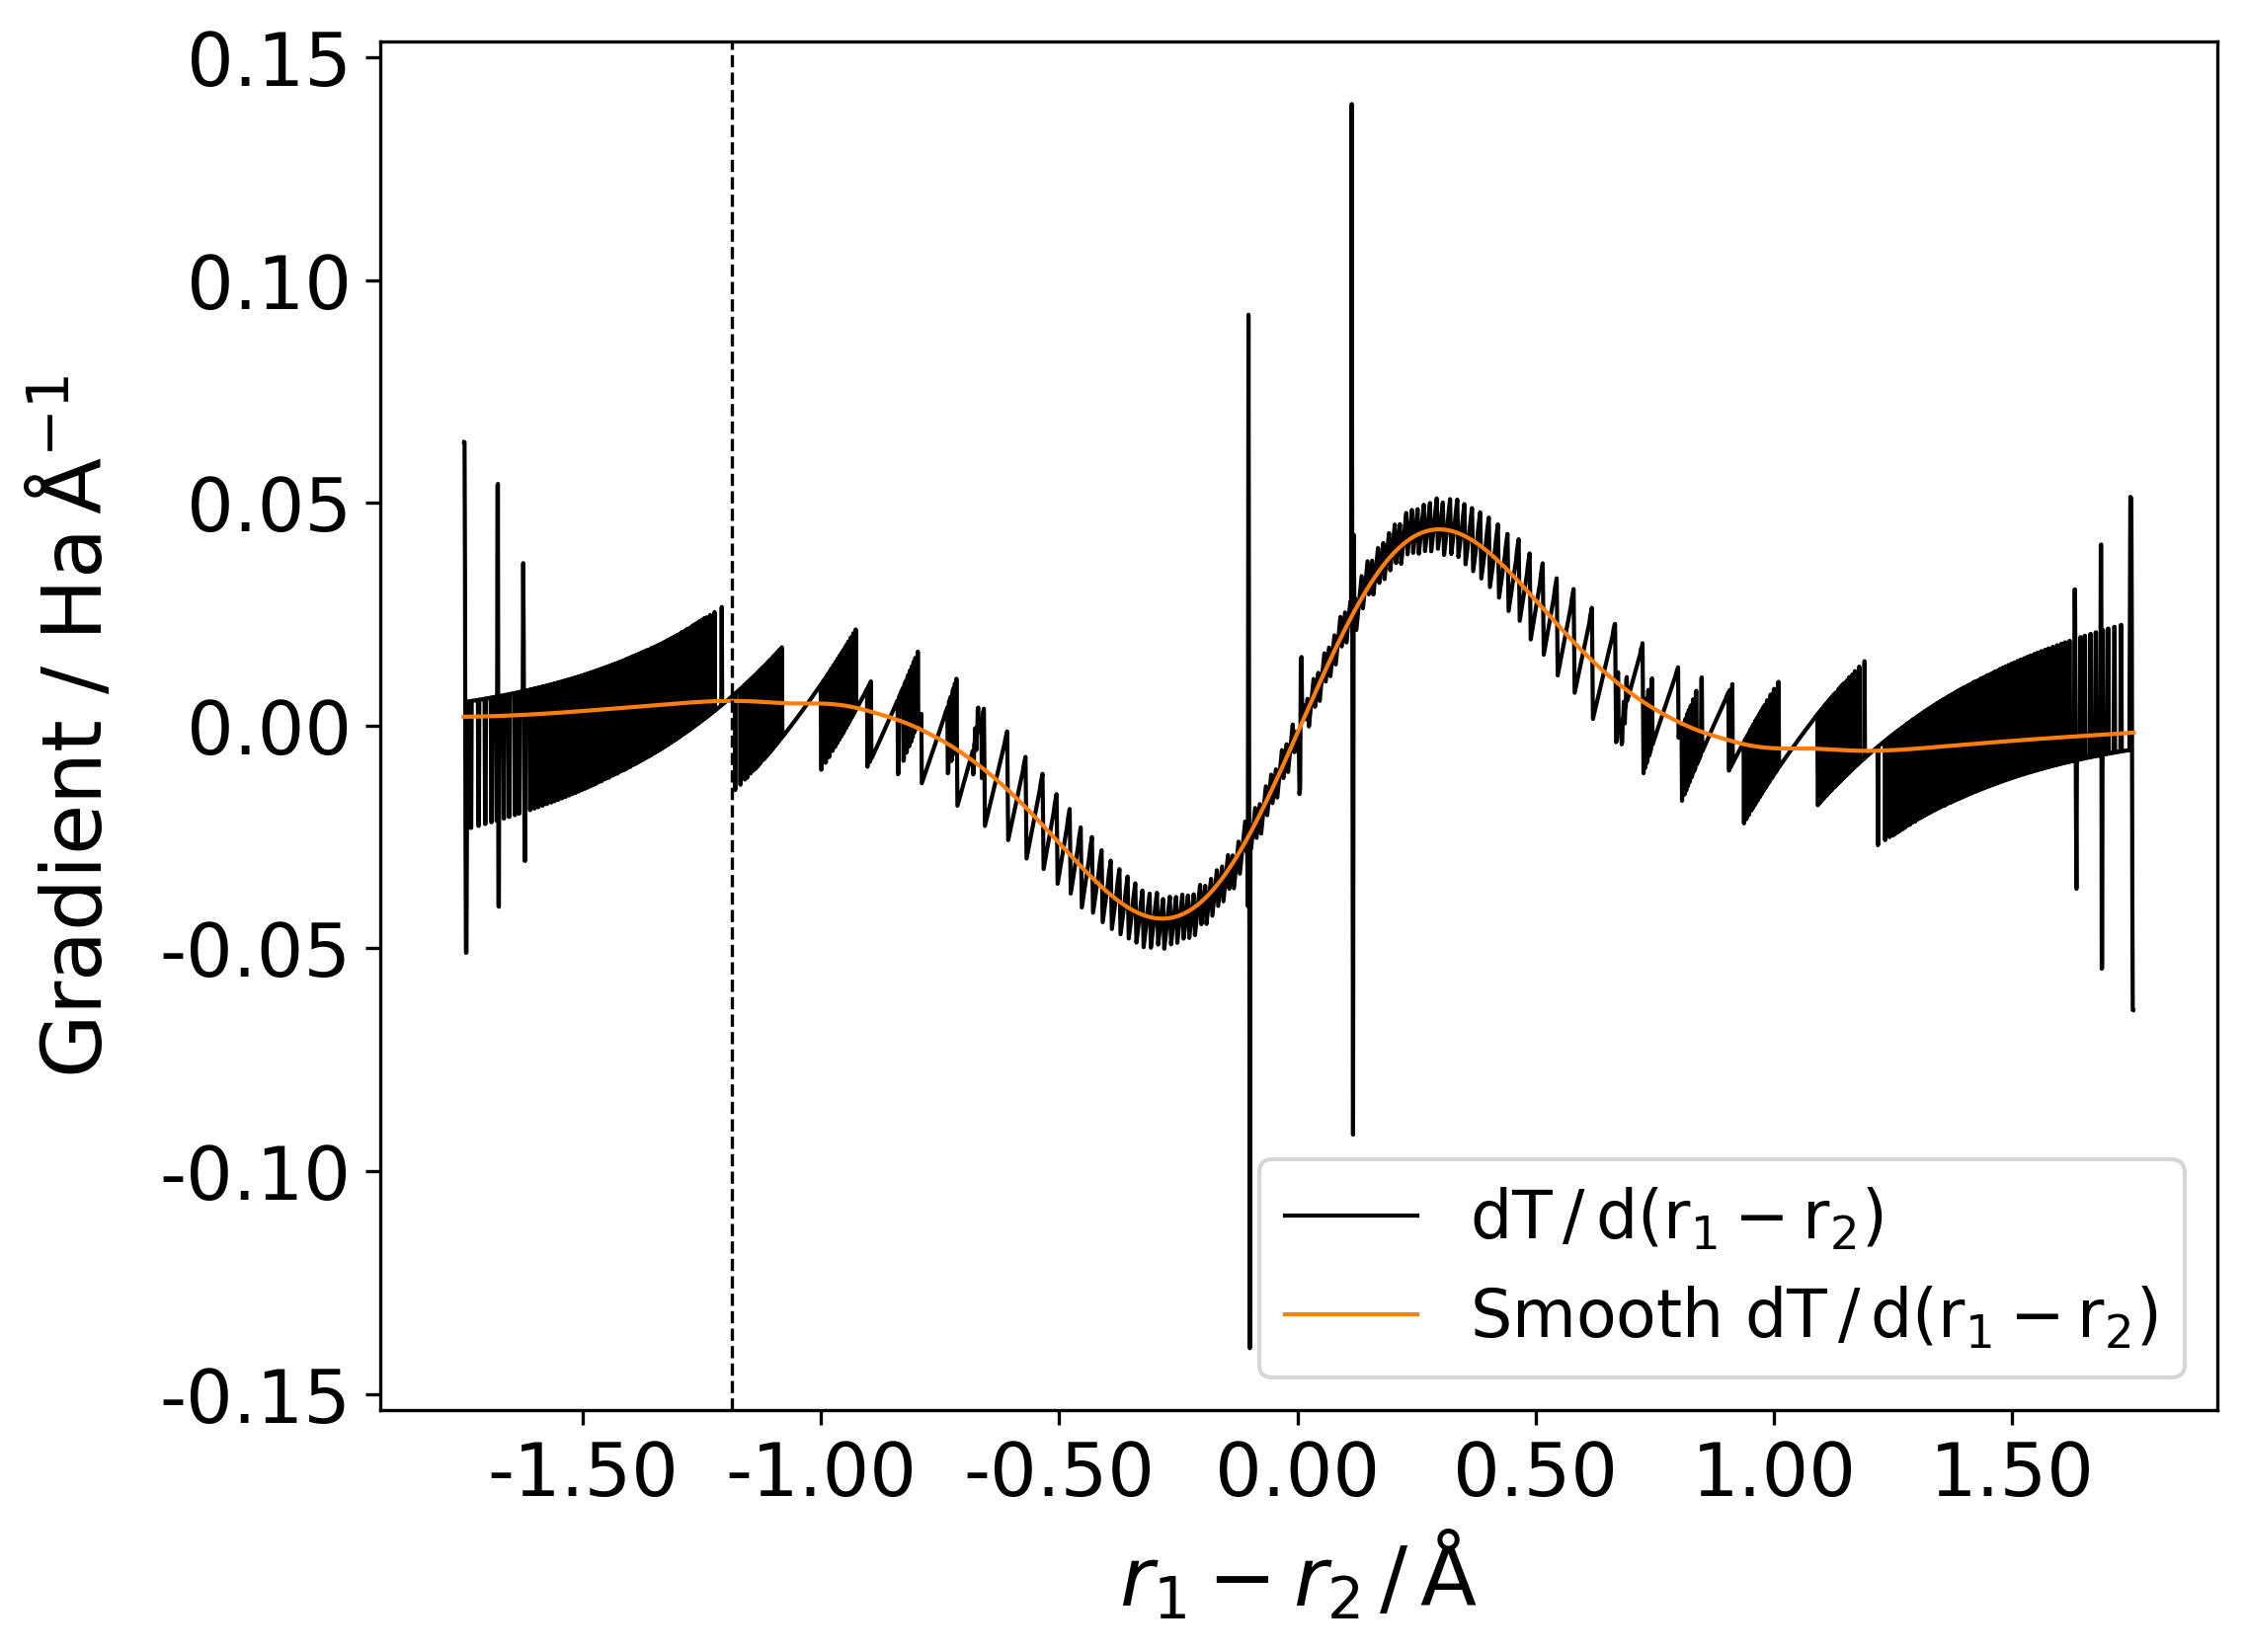
\includegraphics[width=0.9\textwidth]{images/ccsd_pertT_KE_grad.png}
\subcaption{}
\end{subfigure}
\caption{\textbf{(a)} CCSD(T)/aug-cc-pVTZ kinetic energy calculated from the numerical energy gradient and virial theorem, \textbf{(b)} gradient of the kinetic energy and the fitted spline}
\end{figure}

\begin{figure}[H]
\centering
\begin{subfigure}[t]{0.5\textwidth}
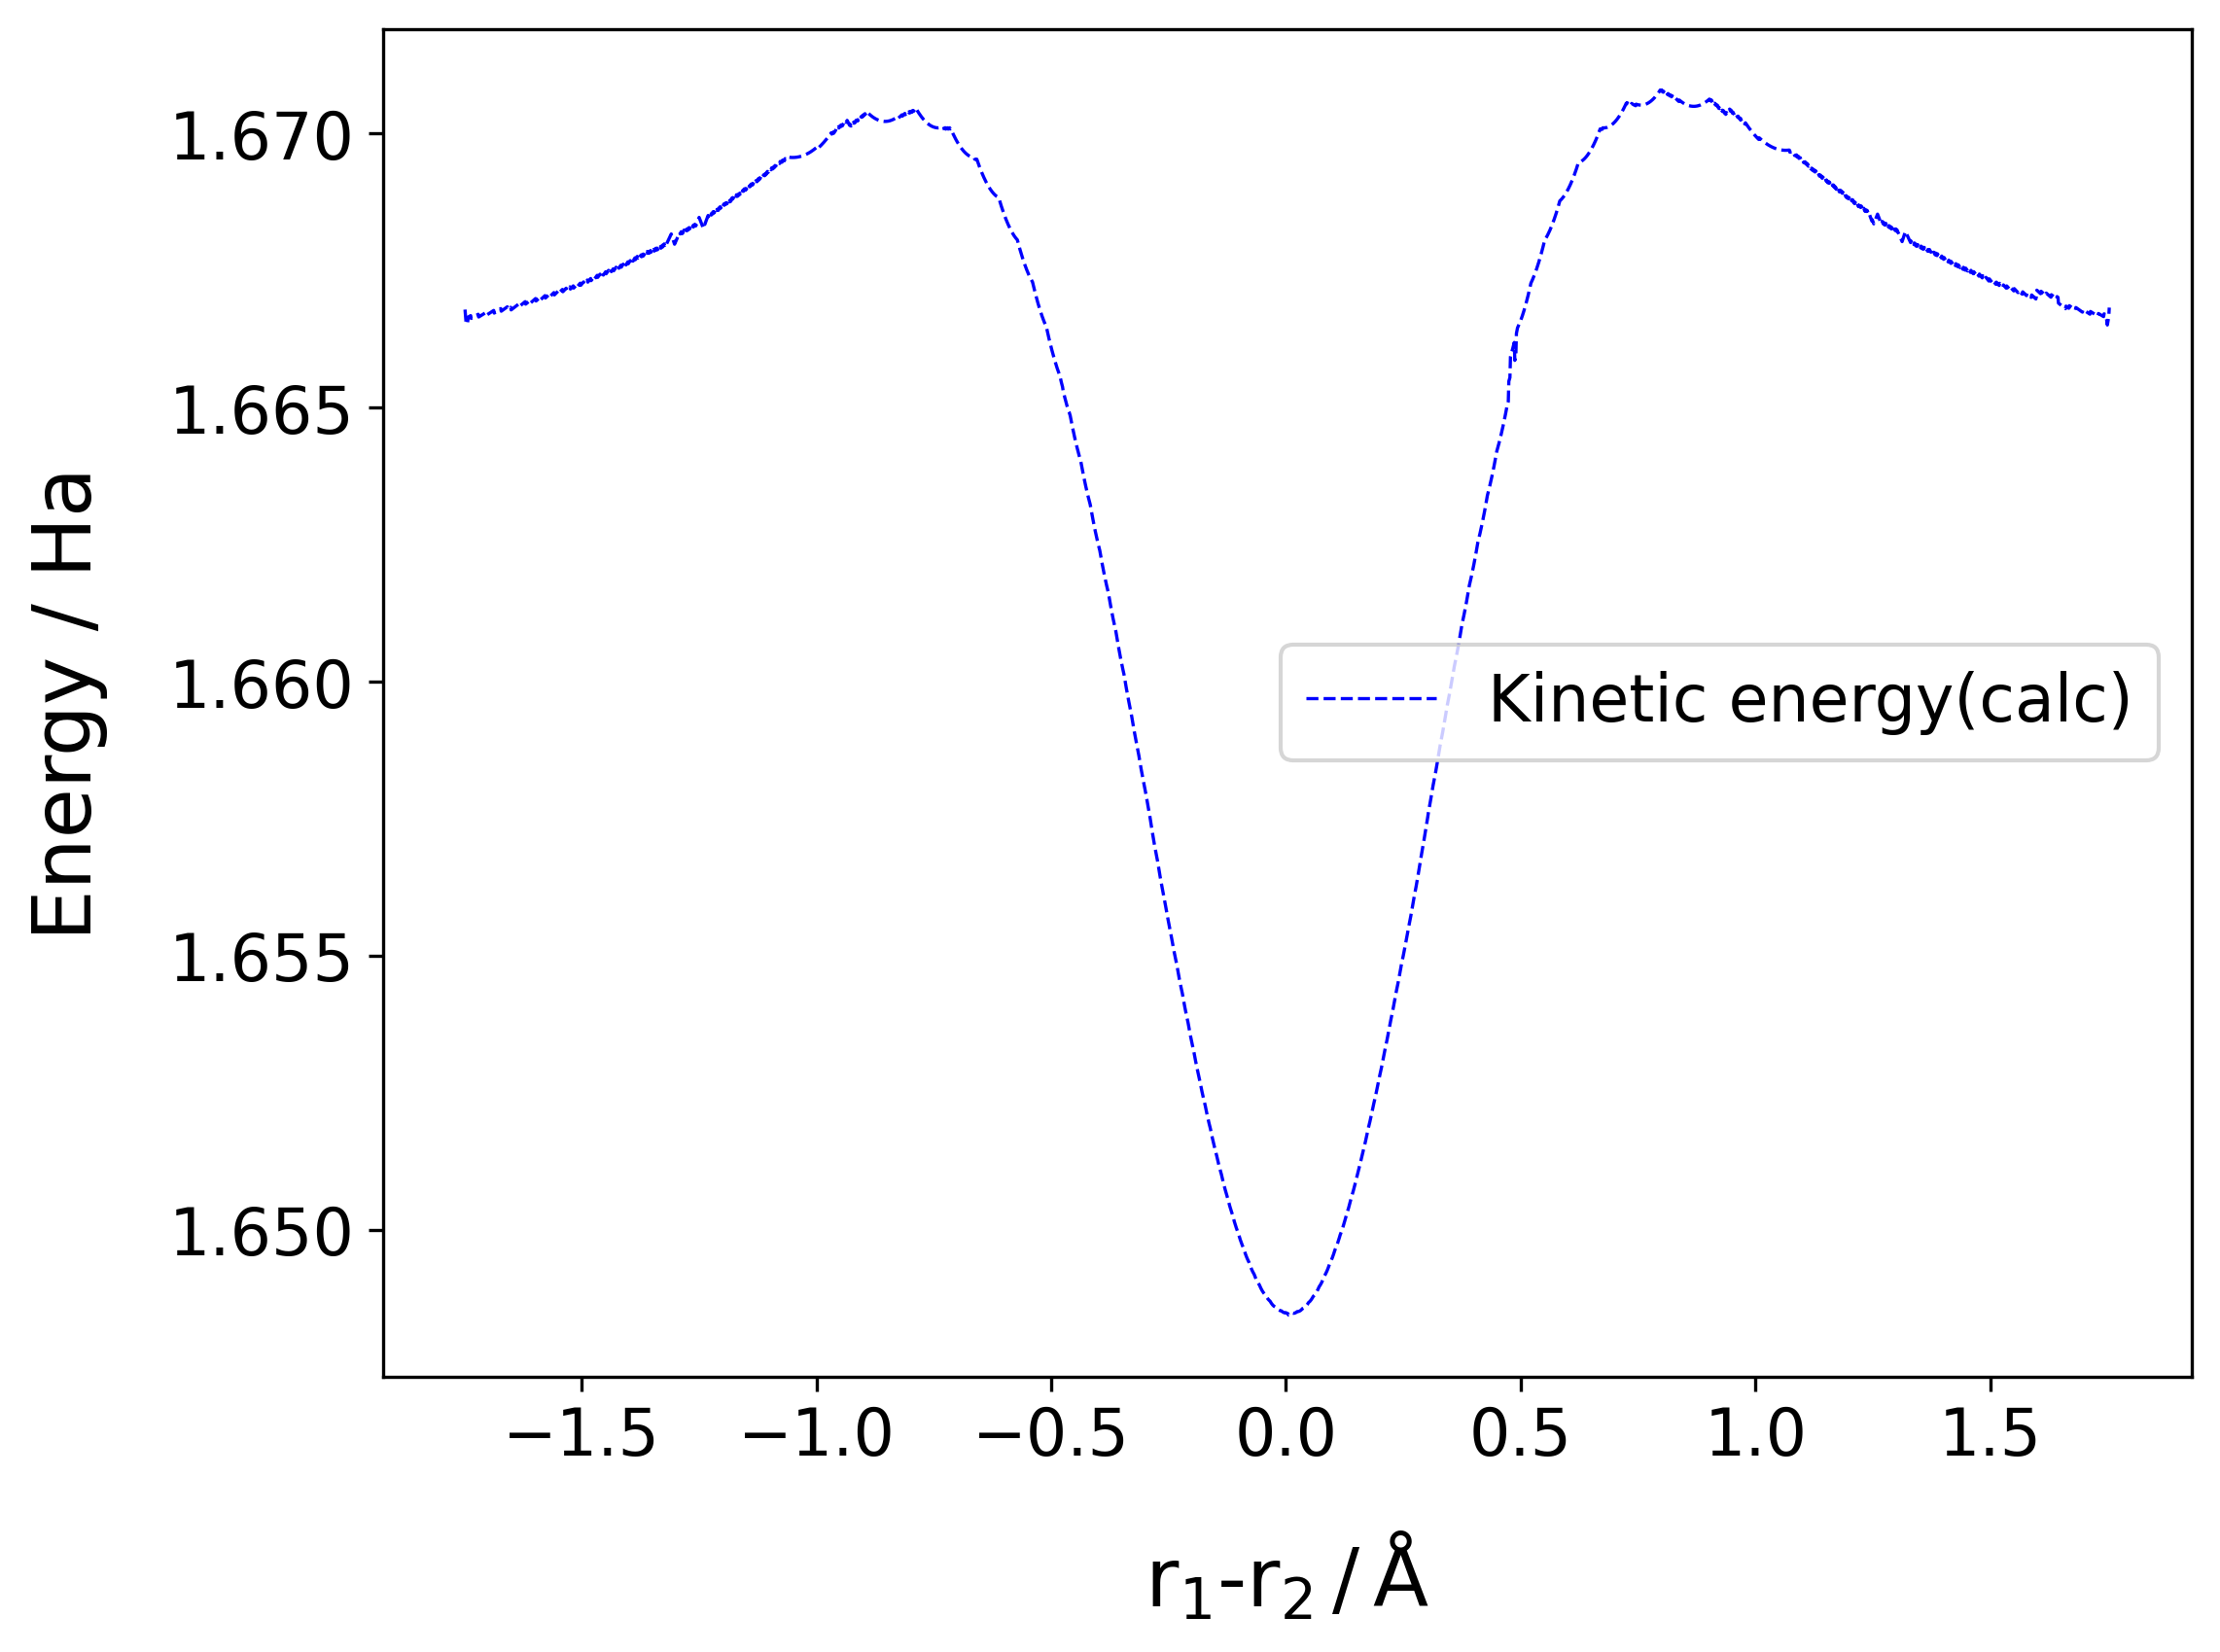
\includegraphics[width=0.9\textwidth]{images/nevpt2_KE.png}
\subcaption{}
\end{subfigure}%
\begin{subfigure}[t]{0.5\textwidth}
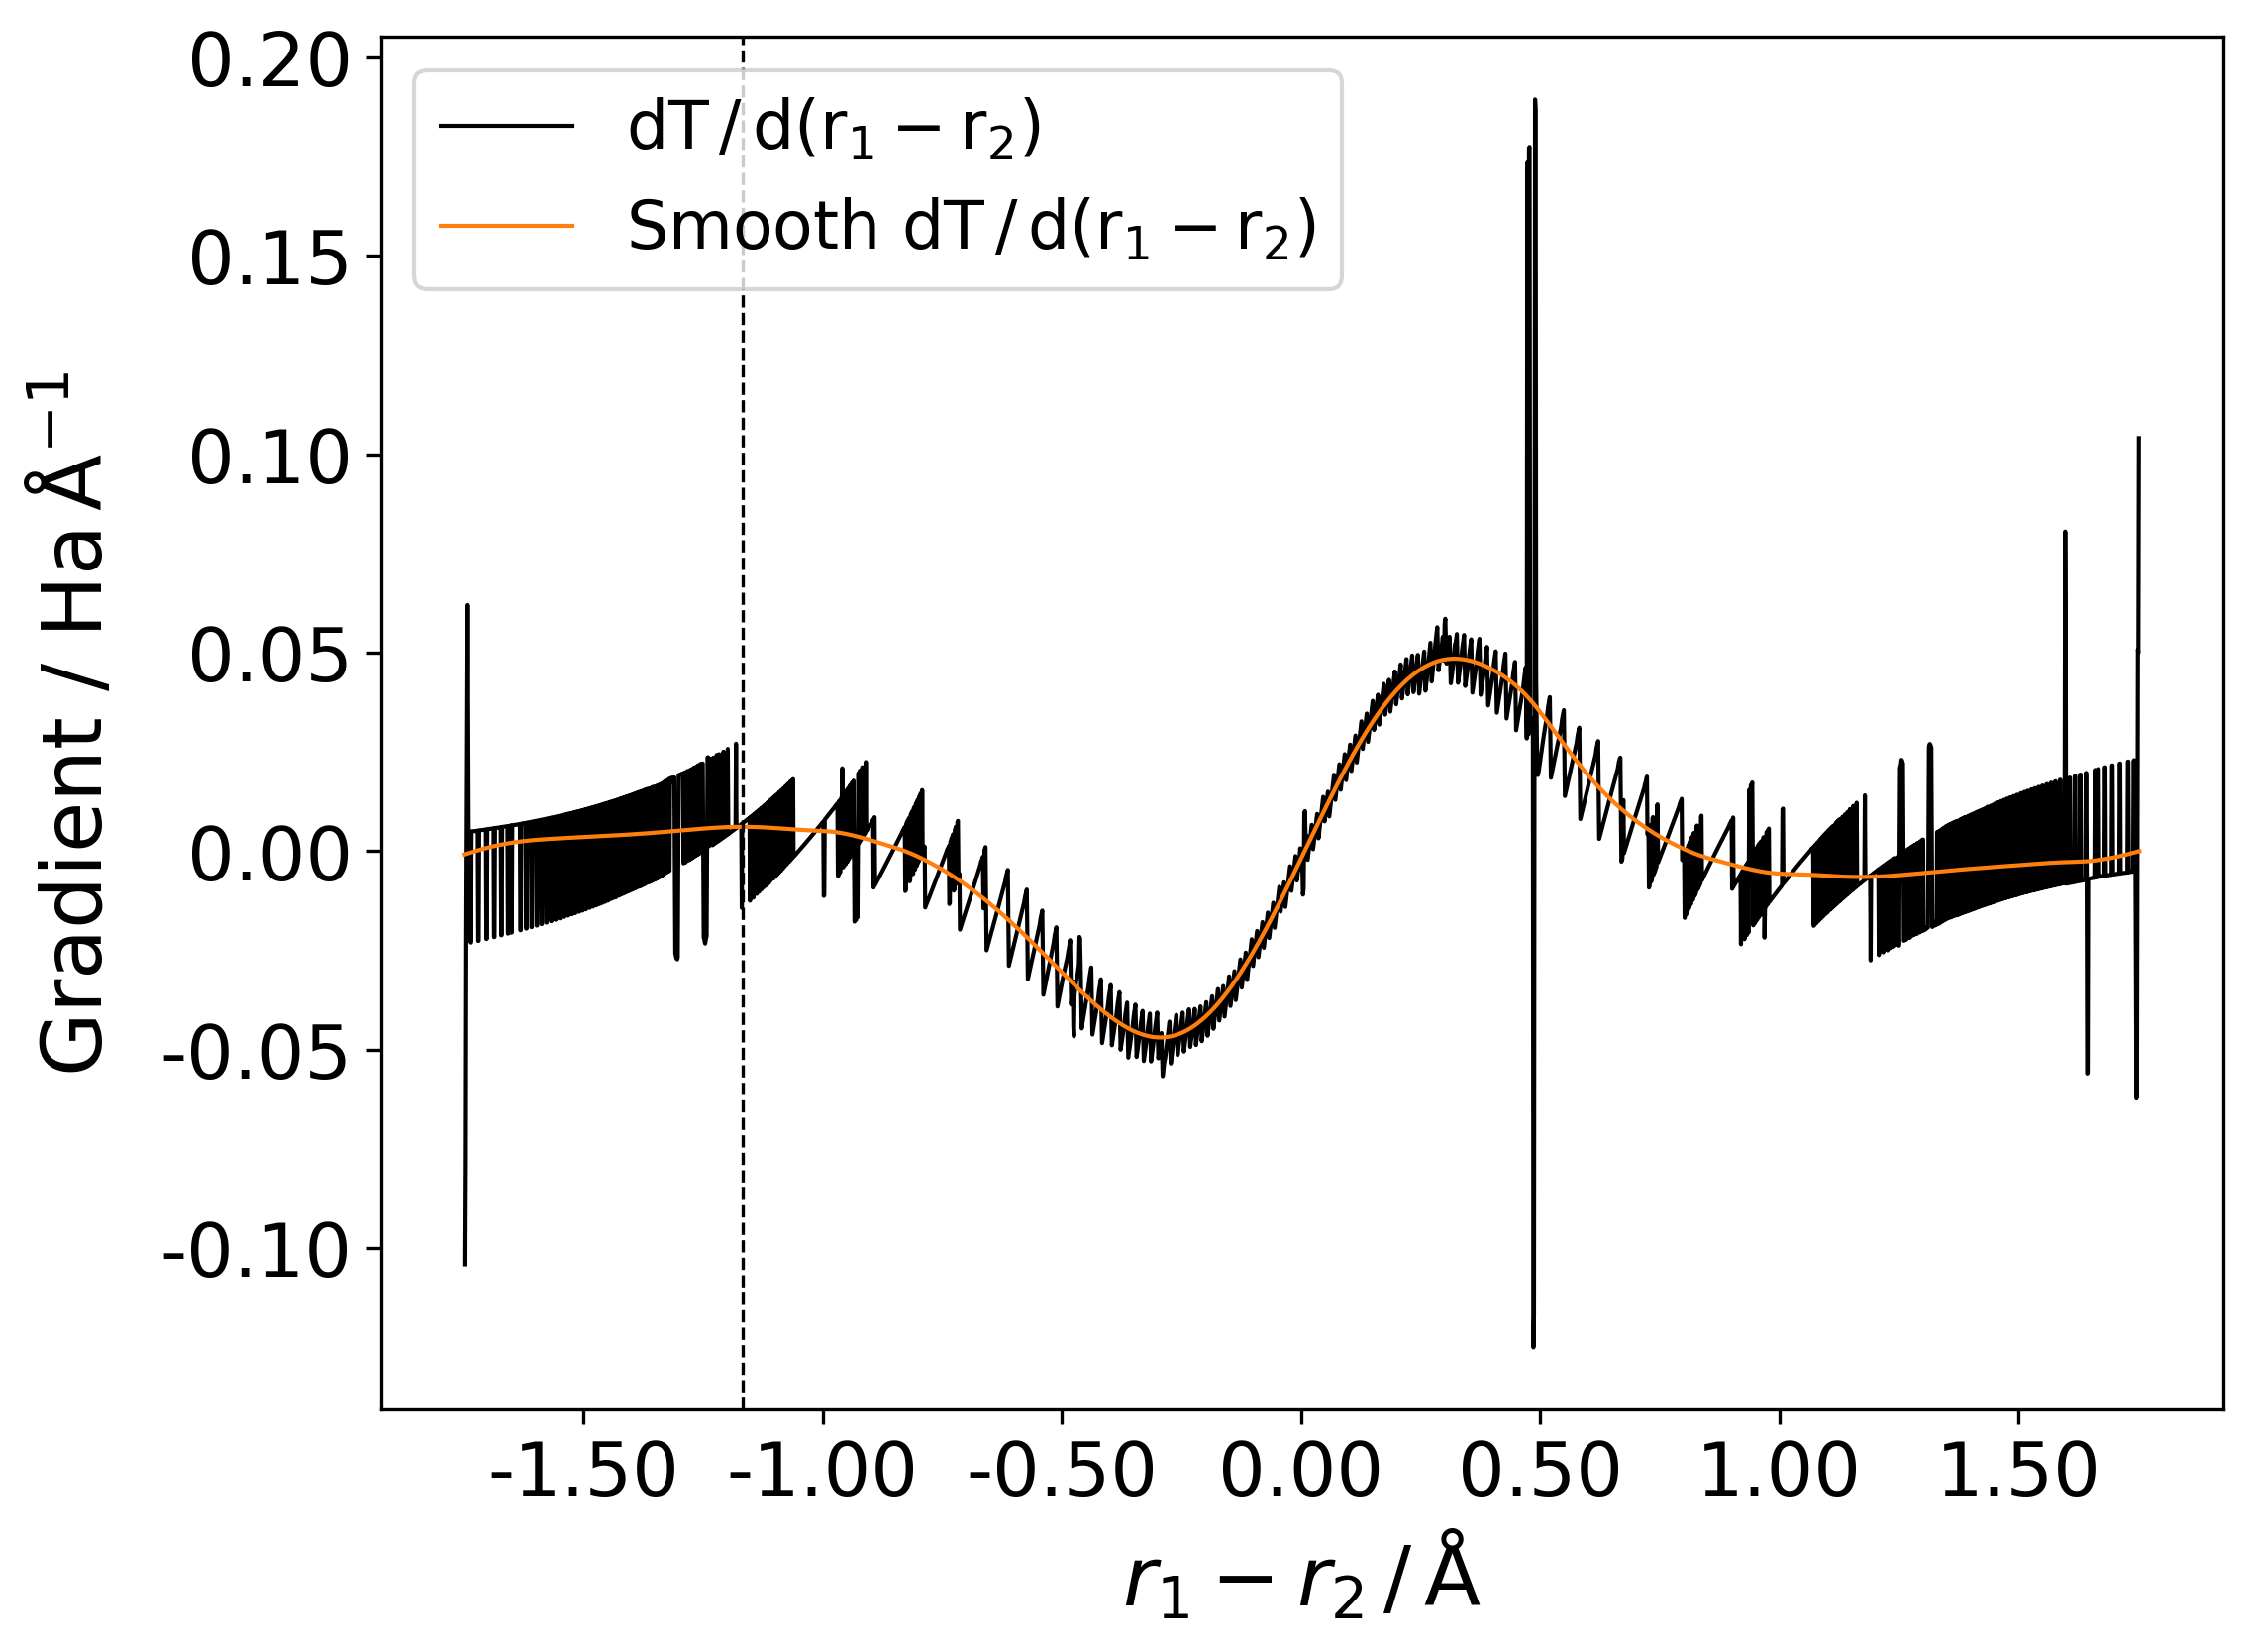
\includegraphics[width=0.9\textwidth]{images/nevpt2_KE_grad.png}
\subcaption{}
\end{subfigure}
\caption{\textbf{(a)} NEVPT2/aug-cc-pVTZ (ORCA 6.0.1) kinetic energy calculated from the numerical energy gradient and virial theorem, \textbf{(b)} gradient of the kinetic energy and the fitted spline}
\end{figure}

\bibliography{refs.bib} 


\end{document}
